%%% Kapitoly
\chapter{Experimenty}
Všechny práce zmíněné v úvodní kapitole, sice používají evoluční algoritmy k vytvoření řízení chování homogenního robotického hejna, tzn. s jedním druhem robotů. V následující kapitole podrobně popíši postup hledání optimální chování pro heterogenního hejna. Optimalizaci jsem navrhl a otestoval na třech rozličných scénářích. Hlavní motivací při tvorbě scénářů bylo vytvořit obtížnější úkoly než se obvykle používají jako například: shlukování, vyhýbání překážkám... Navrhnout je natolik komplexně, aby nebylo možné, že část hejna se nebude podílet na jeho plnění. Také jsem volil scénáře, aby se přiblížily situacím z reálného světa. Každému z nich jsem věnoval samostatnou kapitolu, která zahrnuje popis hlavního úkolu scénáře, seznam robotů i s jejich senzory a efektory, způsob hodnocení fitness,rozdělení do podúkolů s průběhem fitness u ES a DE, vizualizaci a rozbor chování nejlepšího jedince.  
\subsubsection{Pracovní názvy scénářů:}
\begin{enumerate}
	\item Wood Scene - zpracování dřeva
	\item Mineral Scene - přetvoření minerálů na palivo 
	\item Competitive Scene - soubojový scénář
\end{enumerate}
\par
Pro řešení problému jsem navrhl řadu postupů, proto v tomto odstavci zmíním ty nejvíce přímočaré a slibné, které se ovšem ukázaly  jako neúspěšné. V kapitolách zabývajícími se konkrétními scénáři už budu pouze popisovat jen konečné, úspěšné postupy.
 \par
Nedostatečný se ukázal pokus provádět evoluci pro fitness hlavního úkolu scénáře. Konkrétně pro Wood Scene počet natěženého a uskladněného dřeva, pro Mineral Scene objem vytvořeného paliva, pro kompetitivní scénář zbylé body zdraví a udělené poškozený. Většina hodnocení náhodných chování byla rovna nule, proto EA nedostaly dostatek informací k vhodné exploraci a díky malé pravděpodobnosti vygenerování chování alespoň částečně řešící hlavní úkol nedocházelo ani k exploataci. Což mělo za důsledek neefektivní  DE a ES, takže ani jeden z EA nedošel k úspěšnému řešení. 
\par
Posun zaznamenala více obecná fitness i když sama o sobě také nedosáhla do kategorie úspěšných postupů. Do fitness jsem zahrnul i menší pozitivní znaky, které byly součástí hlavnímu úkolu. Například jsem záporně ohodnotil pokusy o pohyb končící kolizí, kladně počet nalezených entit či vhodných objektů v kontejnerech, aktuální stav paliva. Optimalizovaná chování opravdu zaznamenala posun. Ovšem oba EA obtížně hledaly cestu z lokálního optima a ve většině případů optimalizovali pouze jednoduché části úkolu. I přes přidávání složitějších matematických funkcí do fitness nebyly schopny dosáhnout uspokojivého řešení hlavního úkolu scénáře. 
\par 
Pro finální řešení jsem zvolil metodu, kterou nazývám metodou podúkolů. U každého scénáře podrobně popíši její průběh a nastavení, zde pouze nastíním základní  myšlenku. Rozdělil jsem hlavní cíl na několik menších podúkolů (metaúkolů). Každému z nich vytvoříme fitness funkci odpovídající nutné části hlavního cíle. Fitness metaúkolu jsem navrhoval, tak aby necílila na již optimalizované úkony a v každém podúkolu jsem se vždy soustředil pouze na jeden jednoduchý úkon. Díky tomuto principu jsem dosáhl mnohem vyšší odolnosti proti uvíznutí v lokálním minimu. Explorace se tímto procesem také zlepšila, protože hlavní cíl závisí na podúkolech a pokud bylo chování rozmanité a úspěšné, přenesly se tyto vlastnosti i dále. Poté jsem generaci úspěšnou v průzkumu optimalizoval na sbírání materiálů pouze požadované barvy a takto jsem rozděloval až k finálnímu úkolu scénáře. 
\par 
Každý robot má připojen paměťový slot, neboť roboti s nimi dosahovali ve všech úkolech znatelně lepších výsledků a pomáhaly vytvářet složitější chování. 
\section{Použité technologie}
Tuto kapitolu věnuji klíčovým technologiím, jenž jsem použil pro modelování zadaného problému a optimalizaci náhodných chování. Pro ovládání robotů jsem zvolil v poslední době velmi oblíbené \textit{neuronové sítě}, které se často používají v kombinaci s EA. Jednomu jedinci odpovídá jedna neuronová síť ovládající všechny části robota. Tyto neuronové sítě si lze představit jako vektor reálných čísel, což je vhodná reprezentace genotypu pro EA. 
\subsection*{Reprezentace Chování - neuronové sítě}
Pro reprezentaci jedinců v oblasti robotiky, rozpoznávání obrazů a dalších oblastí umělé inteligence se v poslední době používají nejčastěji neuronové sítě. Neuronová síť se strukturou podobá neuronovým sítím v mozku. Základní sítě se skládají z jednotlivých neuronů, které se v kontextu informatického světa nazývají \textit{perceptrony}. Samostatný perceptron je sám o sobě také neuronovou sítí, ale většinou se propojují do složitějších struktur. Perceptron lze definovat podle \citep{neuron} následovně.
\begin{definice}[Perceptron] Perceptron je funkce z $\mathbb{R}^n \rightarrow \mathbb{R}$, která je dáná následujícím předpisem: 	$Y = S(\Theta + \sum_{i=0}^{n} w_i x_i)$, kde pro $i \leq n$ $x_{i}$ je $ítý$ prvek vstupního vektoru, $w_{i}$ se označuje jako váha a většinou $w_{i} $ se bere z $\mathbb{R}$.  $\Theta$ se nazývá práh (bias) a slouží jako váha s konstantním vstupem 1.  $S(X)$ je aktivační funkce: $\mathbb{R} \rightarrow \mathbb{R}$ a $Y$ se obvykle označuje jako výstup perceptronu.
\end{definice}
\textit{Jednovrstvou neuronovou sítí} pak myslíme n perceptronů, tedy funkci $\mathbb{R}^{n} \rightarrow \mathbb{R}^{n}$, kde $ítou$ složku výstupního vektoru dostaneme aplikací funkce odpovídající $ítému$ perceptronu na vstupní vektor.
\improvement{Přidat část o aktivačních funkcích}
\par
Pokud zapojíme z výstupu jednoho perceptronu na vstup jiného, vznikne \textit{vícevrstvá neuronová sít}. Což znamená, že podmnožiny výstupů z první vrstvy neuronů neurčují přímo výstup, ale jsou opět zvoleny jako vstupní vektory pro další jednovrstvou neuronovou síť. Tímto postupem můžeme vytvářet velmi komplexní struktury.
\par
Skrytá vrstva (hidden layer) je taková jednovrstvá neuronová síť, jejíž výstup je pouze vstupem jiných perceptronů.
\par
Pro mé účely se jsem testoval řadu různých variant neuronových sítí, ale nejvíce se mi osvědčilo následující nastavení, které poskytovalo uspokojivé výsledky a rozumné časové nároky. 
\par 
Jako aktivační funkce jednotlivých perceptronů se mi nejvíce osvědčila často používaná funkce hyperbolického tangentu se změněným oborem hodnot pro konkrétní výstup.
\par
V rámci testovaní jsem zvolil jednoduchou architekturu jednovrstvé neuronové sítě, což se ukázalo jako dostatečné pro uspokojivé řešení jednotlivých scénářů. Jejich architektura je následující. Pro každé reálné číslo, které očekává robot jako vstup pro efektor, byl připojen perceptron do kterého vstupuje vektor reálných čísel odpovídající vektoru všech hodnot přečtených ze senzorů.  Pro dosažení lepších řešení by zde bylo možné nasadit NEAT algoritmus či hledat více specifičtější architektury.Případně vyzkoušet vliv vícero vrstev. \improvement{Přidat do diskuze}
\subsection*{Evoluční algoritmy}
Neuronovou sít si lze představit jako množinu vektorů, kde jeden perceptron odpovídá vektoru reálných čísel (vah vstupů + práh $v =(x_0,x_1...x_n,\Theta)$. V kontextu evolučních algoritmů se pro optimalizaci vektorů reálných čísel nejčastěji používají ES a DE, I z tohoto důvodu jsem zvolil zmíněné algoritmy jako zástupce pro optimalizaci chování heterogenní skupiny robotů. Oba zmíněné algoritmy důkladně popisuji v kapitole \ref{sec:DE} a \ref{sec:ES} a má implementace se od popisu v úvodu liší pouze v malý detailech. Do detailu si je lze prohlédnout v přiložené dokumentaci a kódu. 
\par
V rámci testovaní jsem vyzkoušel mnoho různých nastavení parametrů EA. V tabulce níže jsou uvedeny nakonec použité parametry, které dosahovali v experimentech největších úspěchů. Jedná se o tradičně používané parametry, osvědčené v řadě optimalizačních problémů. 
\begin{table}[h]\centering
	\subsubsection{Nastavení parametrů}
	\begin{tabular}{l@{\hspace{1.5cm}}D{.}{,}{3.2}D{.}{,}{1.2}D{.}{,}{2.3}}
		\toprule
		 \textbf{differenciální evoluce}\\
		\midrule
		F:     & 0.8 \\
		CR:  & 0.5 \\
		\toprule
		\textbf{evoluční strategie}\\
		\midrule
		alpha & 0.05 \\
		sigma & 0.1\\
		\bottomrule
		\multicolumn{2}{l}{}
	\end{tabular}
	\caption{Nastavení parametrů u EA}
\end{table}
\newpage
\section{Wood Scene experiment}
Vzorem Wood Scene scénáře byla těžba dřeva, představme si dřevorubce s motorovou pilou a silné dělníky nakládající zpracované stromy do transportérů a svážející materiál na společnou hromadu. Roboti odpovídají těmto lidským rolím, samozřejmě je jejich činnost značně zjednodušena. V obou případech je cílem maximalizovat počet zpracovaného dřeva na daném místě, což vyžaduje od obou druhů agentů spolupráci. \par
Robotické hejno se ve Wood Scene snaží natěžit a převést, co největší množství dřeva na místo označené rádiovým signálem. Rádiové senzory poskytují robotům sílu signálu a vysílaný kód. Pro místo určené na kupení dřeva je určen unikátní kód 2 a je umístěn doprostřed mapy. Žádný jiný rádiový vysílač vysílající signály s kódem 2 se na mapě nenachází.  
\par
Celé hejno čítá 9 robotů, jedná se o dva různé druhy, které se liší velikostí, rychlostí, senzory i efektory. Při začátku experimentu jsou náhodně rozmístěny do středu mapy na stejné místě jako se rozprostírá skládací prostor. Dále jsou na mapě náhodně umístěny stromy. Robot v kontextu scénáře nazývaný Scout odpovídá \uv{dřevorubci} v teoretickém vzoru, pohybuje se rychle, má menší rozměry, umí nalezený strom zpracovat na dřevo pro komunikaci má přidělený unikátní kód 0. Oproti tomu robot \uv{dělník} se pohybuje pomaleji, je větší, neumí zpracovávat stromy, ale disponuje nakladačem (vykladačem) a kontejnerem na 5 objektů. 
 \par 
Souhrnně hejno musí strom nalézt, přepracovat na dřevo, poté naložit a odvézt do středu. Celý tento proces zahrnuje typické úkoly pro robotický swarm jako rozprostření, vyhýbání se překážkám, komunikaci mezi jednotlivými agenty, nalezení cesty apod. Z návrhu je zřejmé, že na procesu se musí podílet oba druhy robotů.
\par
V rámci bakalářské práce byla připraven program zajišťující jednoduchou vizualizaci chování robotů. Jeho vizuální výstup můžete vidět na obrázku \ref{obr04:WoodSceneRandomStart}. Na ní si vysvětlíme jednotlivé entity nacházející se na mapě. Mapa je ohraničena obdélníkovou hranicí a chová se jako zeď. Zelené kroužky znázorňují stromy, které ještě nebyly objeveny. Oxbjevený strom změní barvu na žlutou. Modře označený prostor je určen pro uskladnění zpracovaného dřeva, roboti jej zaznamenají jako rádiový signál. Hnědá kolečka zastupují pokácené dřevo. V některých podúkolech se objevuje dřevo už při inicializaci, proto ještě neobjevené má tmavší barvu a objevené světlejší. Pro roboty je v tomto prostoru vysílán rádiový signál. Roboti jsou vyplněny červenou barvou, jejich senzory a efektory mají černou barvu. Pro každý rádiový signál je určena jedna unikátní barva s alfa kanálem. 
\par
Pro potvrzení, že scénář není triviálně řešitelný. Bylo vygenerováno tisíc náhodných chování. Hodnoceny byly dle fitness funkce podúkolu kooperace popsaný níže. Nejlepší z nich můžete vidět těsně po inicializaci mapy \ref{obr04:WoodSceneRandomStart}. Výsledek krátce před 10 000 iterací je zachycen v obrázku \ref{obr04:WoodSceneRandomEnd}.

\begin{figure}[p]\centering
	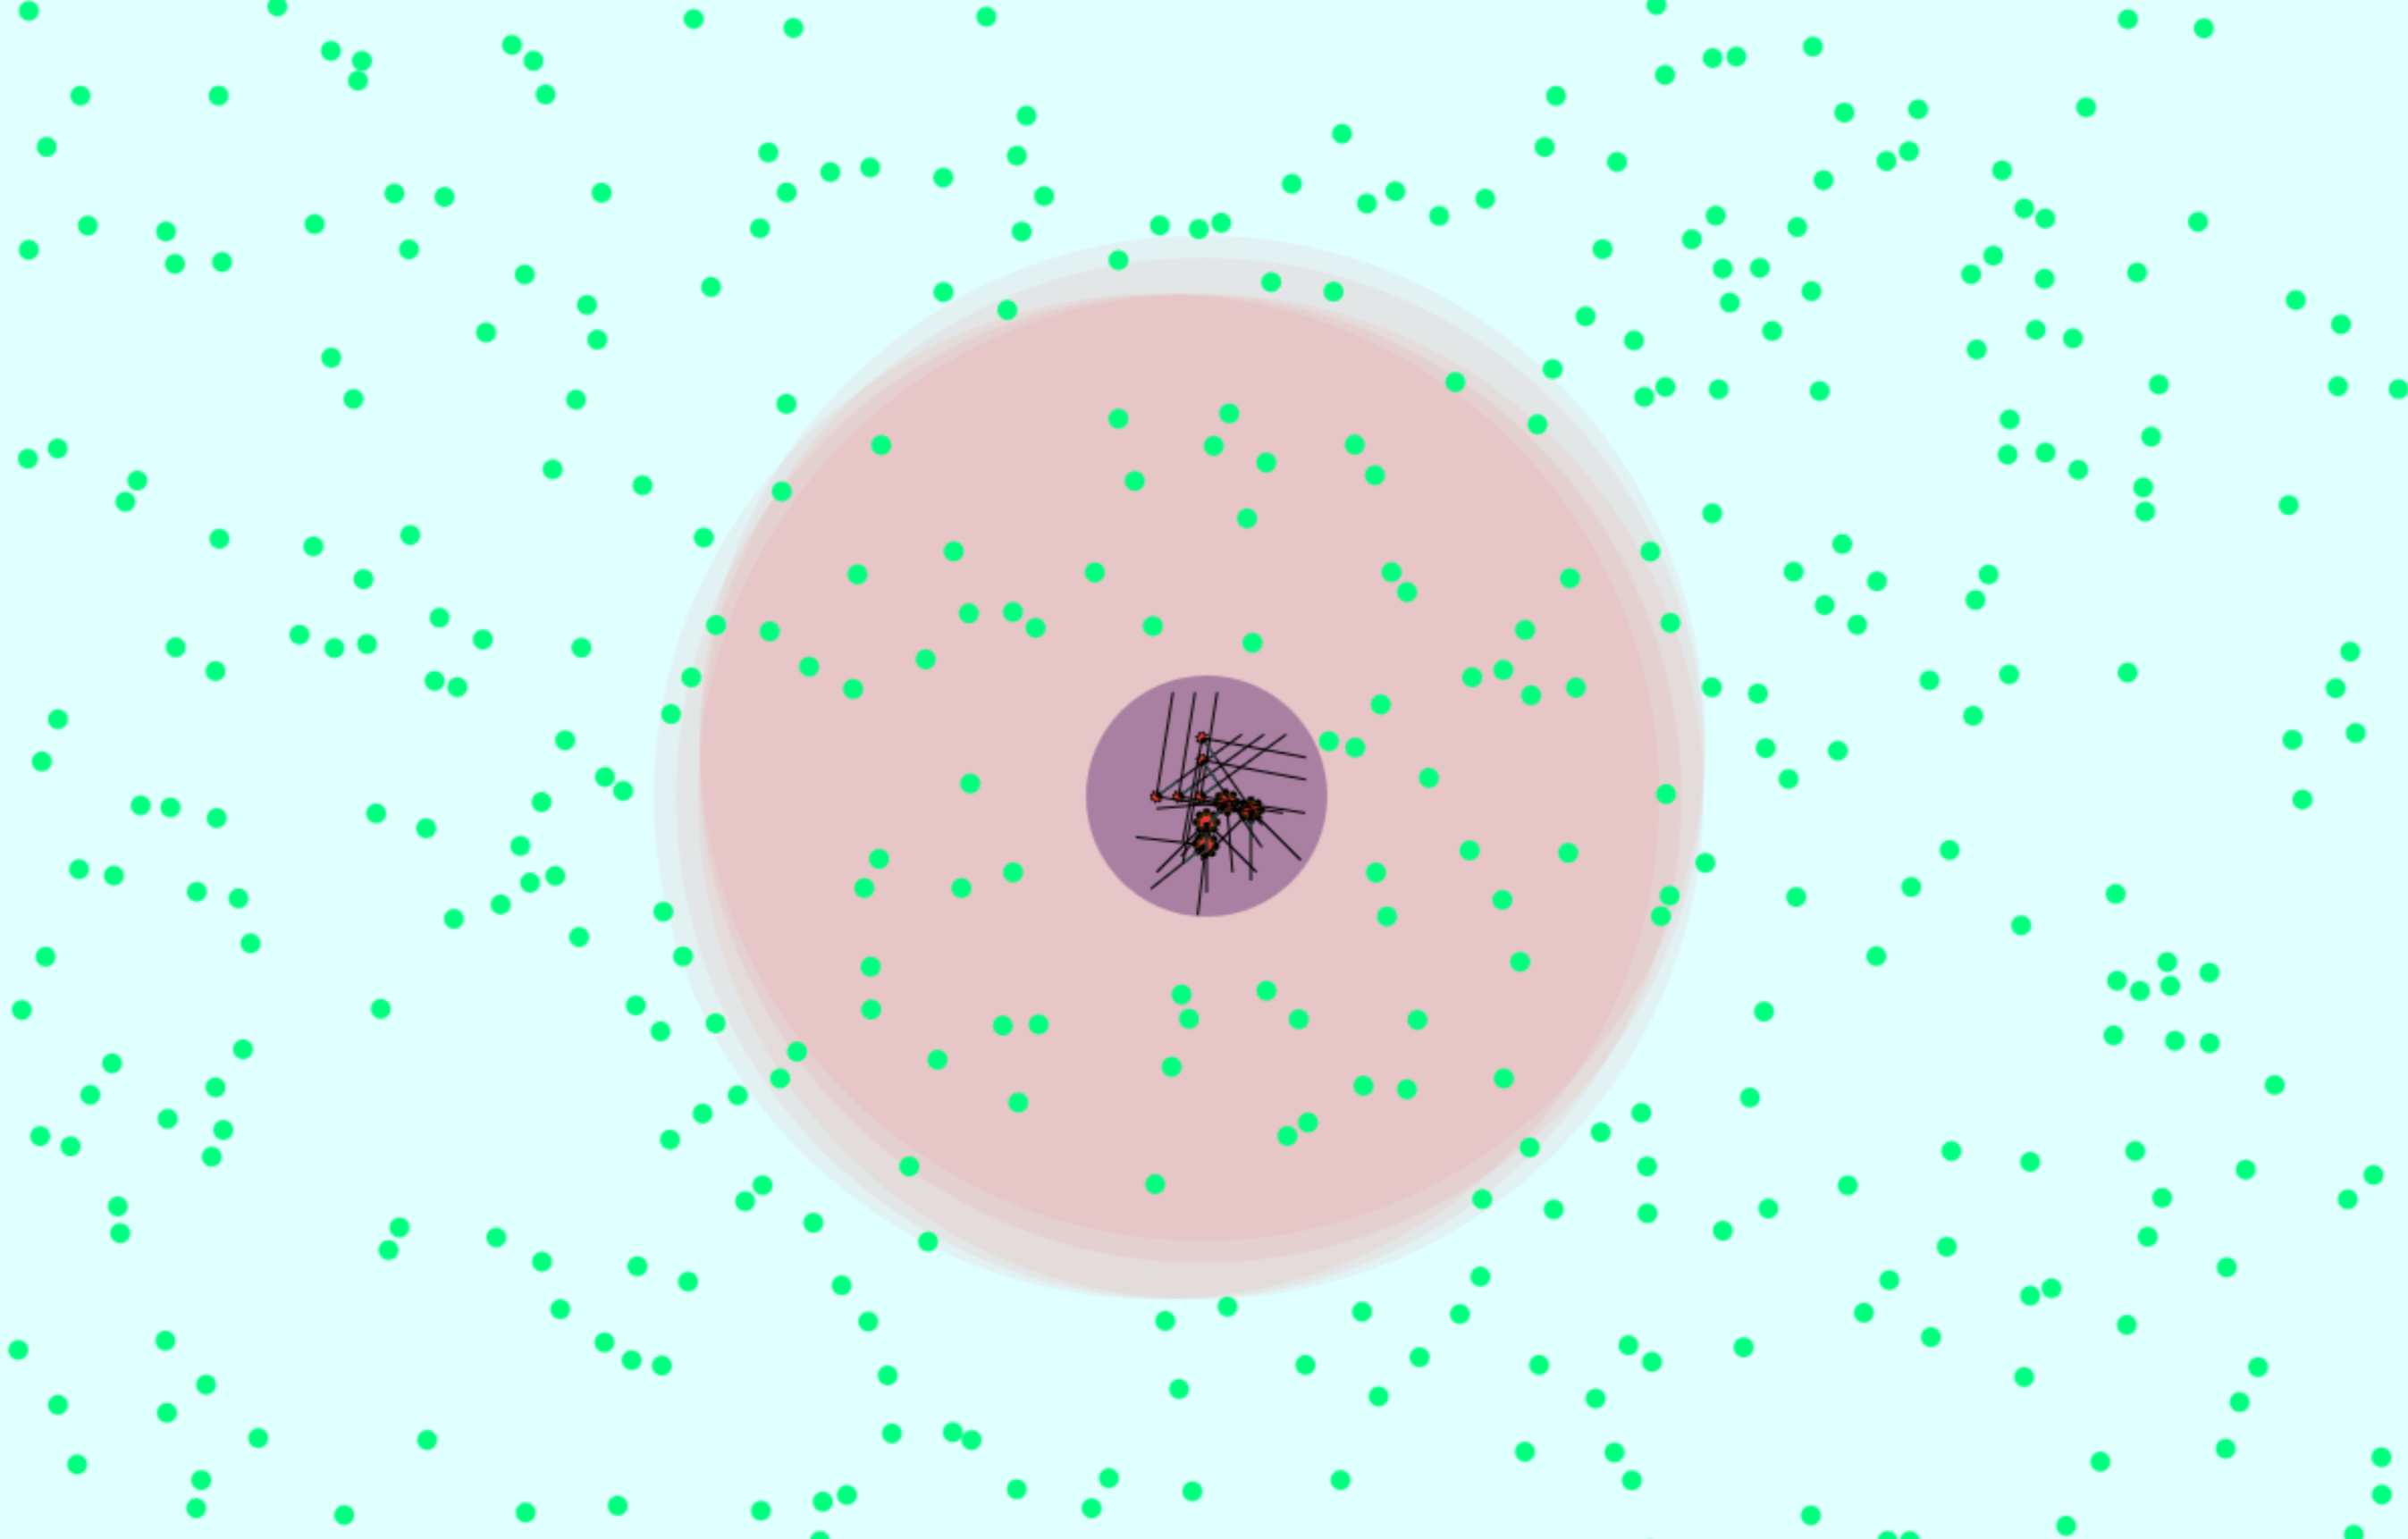
\includegraphics[width=\columnwidth]{../img/WoodMap/pictures/StartRandom.png}
	\caption{Příklad WoodScene mapy: start náhodného chování}
	\label{obr04:WoodSceneRandomStart}
\end{figure}
\par

\begin{figure}[p]\centering
	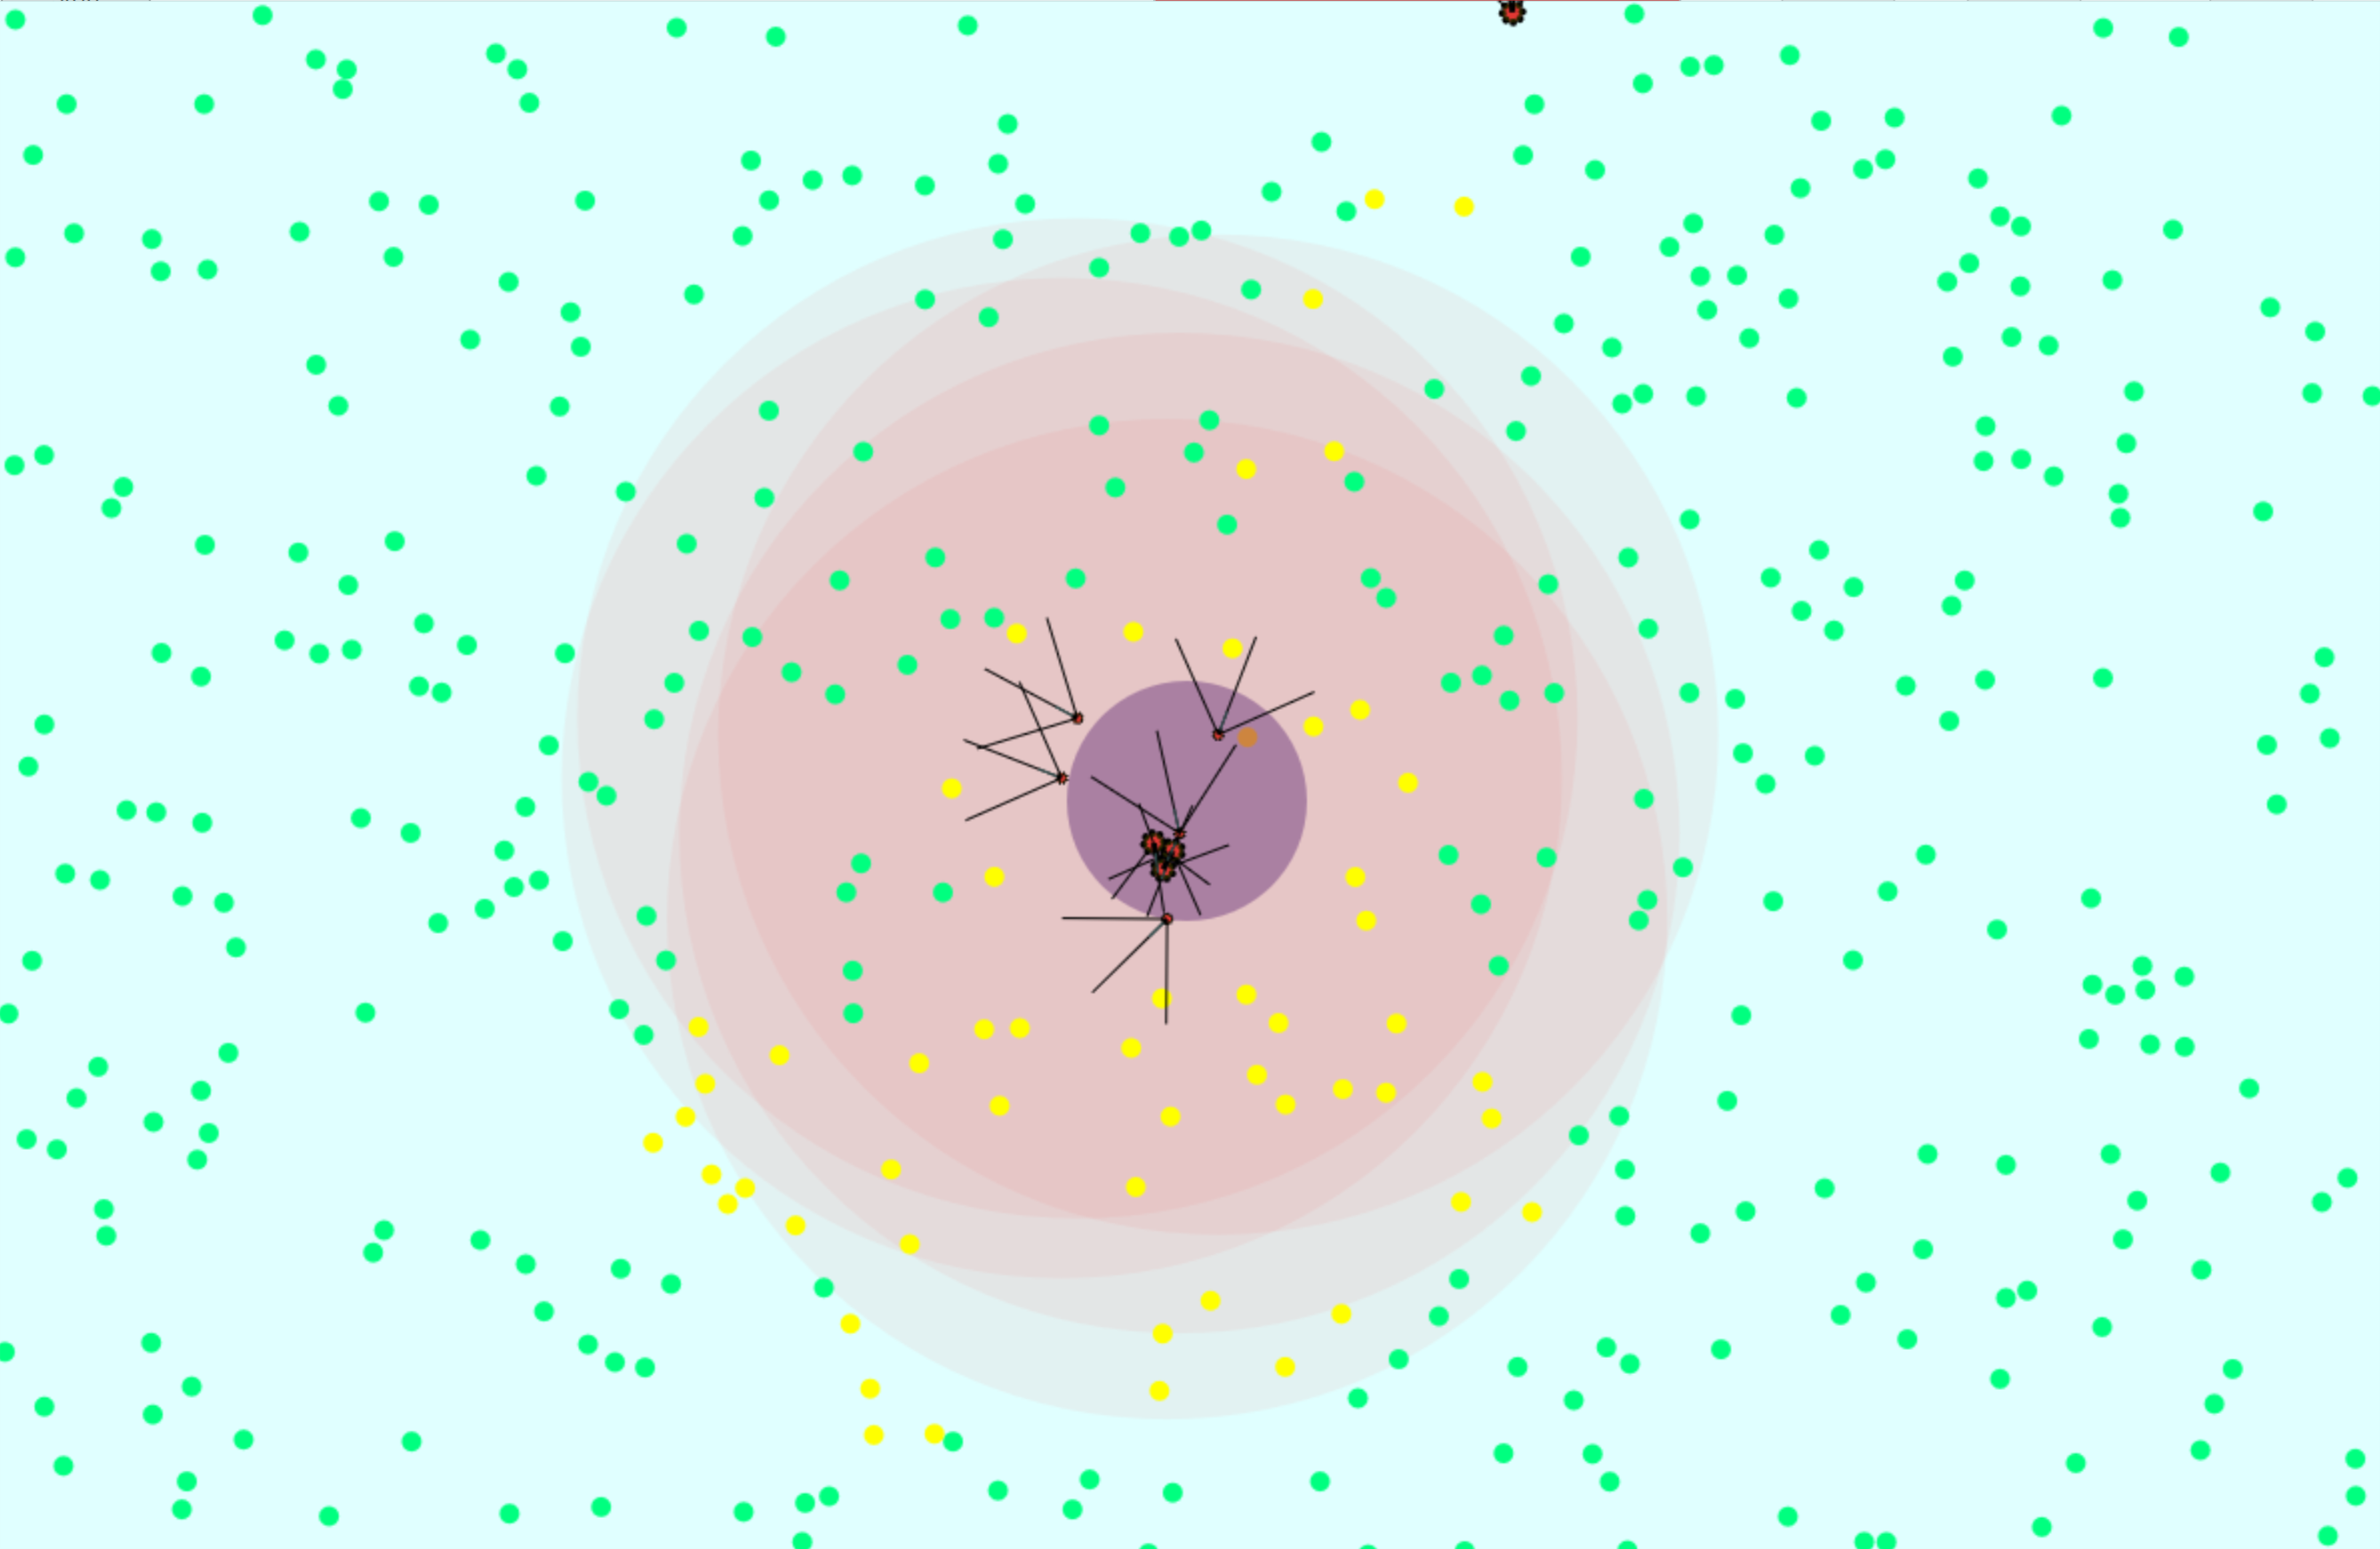
\includegraphics[width=\columnwidth]{../img/WoodMap/pictures/EndRandom.png}
	\caption{Příklad WoodScene mapy: po 9000 iteracích náhodného chování}
	\label{obr04:WoodSceneRandomEnd}
\end{figure}
\clearpage
\subsection{Roboti}
Devítičlenné hejno obsahuje 5 Scout robotů a 4 Worker roboty. U každého z robotů popíši jejich efektory a senzory. Pro každý druh robota je připravena jedna shodná neuronové sítě. Jedinec odpovídá dvojici neuronových sítí, jedné pro Scout robota a druhé pro Worker robota. Proto fitness funkce hodnotí jejich výsledné snažení dohromady a evoluční operátory pracují nad celou dvojicí. Podívejme se na jednotlivé druhy podrobně.
\subsubsection{Scout robot}
Jedná se o robota, který má na starosti průzkum mapy a kácení nalezených stromů. Na zpracování dřeva používá efektor, nazývám jej refaktor, který má podobu úsečky a vyčnívá z čela robota. Pro zpracovaní musí refaktor kolidovat se stromem v mapě, poté je strom prohozen za entitu dřeva. Aby mohl komunikovat má přidělený rádiový signál s kódem 0, při jeho vysílání přidá na mapu signál jako kruh se středem odpovídajícím pozici robota. Jedná se o menšího robota, oproti Worker robotovi je rychlejší a jeho senzory mají větší dosah. Tabulka obsahuje základní charakteristiky, počty a dosahy jednotlivých senzorů a efektorů
\par 
\begin{table}[h]\centering
\begin{tabular}{l@{\hspace{1.0cm}}D{.}{,}{2.2}D{.}{,}{2.2}D{.}{,}{2.3}}
	\toprule
	\textbf{Scout Robot} \\
	\midrule
        Tvar: & Kruh & \\
        Poloměr: & 2.5 \\
        Název: & WoodCutterM \\
        Velikost kontejner: & 0\\
        \hline
        \textbf{Efektory} \\
        \midrule
        Motor: & Dvou kolečkový \\
        Maximální rychlost: & 3 \\
        Kód rádiového signálu: & 0 \\
        Poloměr signálu: & 200\\
        Refaktor: & Strom \Rightarrow Dřevo \\
        Dosah refaktoru: & 10\\
        Počet paměťových slotů: & 10 \\
        Obsah slotu: & float\\
        \hline 
        \textbf{Senzory} \\
        \midrule
        Počet line senzorů: &  3 \\
        Délka line senzorů: & 50\\
        Orientace line senzorů: & 0^\circ, 45^\circ, -45^\circ \\
        Poloměr type senzoru: & 50\\
        Poloměr rádiového přijímače: &  100 \\
        Počet touch senzorů: & 8 \\  
        Lokátor senzor\\ 
	\bottomrule
	\multicolumn{2}{l}{}
\end{tabular}
\caption{Wood - Scout robot popis}
\end{table}
\clearpage
\subsubsection{Worker robot}
Worker robot se stará o manipulaci a následný transport objektů na mapě. Pohybuje se pomaleji než Scout a také je o něco rozměrnější. Picker, úsečkový efektor sloužící pro nakládání a vykládání objektů, funguje na podobném principu jako refaktor pro naložení musí kolidovat s objektem a pro vyložení s ním nesmí nic kolidovat. Ke komunikaci mu byl vyhrazen rádiový signál s kódem 1. Sebrané objekty ukládá do kontejneru, kam se vejde celkem 5 entit a vykládat umí pouze entitu na vrchu. Tabulka níže popisuje další podrobnosti.
\par 
\begin{table}[h]\centering
	\begin{tabular}{l@{\hspace{1.0cm}}D{.}{,}{2.2}D{.}{,}{2.2}D{.}{,}{2.3}}
			\toprule
			\textbf{Worker Robot} \\
			\midrule
                Tvar: & Kruh\\
                Poloměr: & 5\\
                Název: & WoodWorkerM \\
                Velikost kontejner: & 5\\
                \hline
                \textbf{Efektory} \\
                \midrule
                Motor: & Dvou kolečkový \\
                Maximální rychlost: & 2 \\
                Kód rádiového signálu: & 0\\
                Poloměr signálu: & 200\\
                Dosah pickeru: & 10\\
                Počet paměťových slotů: &10 \\
                Obsah slotu: & float\\
                \hline 
                \textbf{Senzory} \\
                \midrule
                Počet line senzorů: &  3\\
                Délka line senzorů: & 30\\
                Orientace line senzorů: & 0^\circ, 45^\circ, -45^\circ\\
                Poloměr rádiového přijímače: & 100 \\
                Počet touch senzorů: & 8 \\  
                Lokátorový senzor\\ 
	\bottomrule
\multicolumn{2}{l}{}
\end{tabular}
\caption{Wood - Worker robot popis }
\end{table}
\clearpage
\subsection{Vyhodnocování Fitness}
Fitness funkce pro ohodnocení WoodScene scénáře probíhá vždy až na konci simulace. I když se úspěšnost v podúkolech  vždy posuzuje jinak, celou fitness funkci lze shrnout do následujícího cílů. Roboti jsou odměňováni za: 
\begin{enumerate}
        \item nalezené stromy = stromy o které zavadil line senzor 
        \item pokácené stromy = stromy, které refaktor změnil 
        \item sebrané dřevo = zpracované dřevo, které mají roboti uvnitř kontejnerů 
        \item uskladněné dřevo = dřevo, které dovezli na vyznačené místo 
\end{enumerate}
Trestáni za:
\begin{enumerate}
	\item kolize = počet pokusů o pohyb při kterém by došlo ke kolizi 
\end{enumerate}

\subsection{Podúkoly} 
Pro oba použité algoritmy jsem používal stejné úlohy pro naučení robotů postupně těžších a těžších cílů. Hlavně také, abych mohl porovnat oba evoluční algoritmy.  
\begin{enumerate}
        \item vygenerování robotů = Na začátku je vygenerováno chování robotů naprosto náhodně. Pro každého robota, je vygenerována náhodná jednovrstvá neuronová síť. 
        \item učení chůze = Pro oba roboty je velmi důležité, aby se pohybovali bez kolizí po celé mapě a objevovali, co největší prostor. Roboti jsou vyvíjeni odděleně a fitness se soustředí na počet kolizí (záporným ohodnocením) a na nalezené stromy (kladným ohodnocením).
        \item těžba stromů = Scout roboty, kteří se už obstojně po mapě pohybují, je třeba naučit kácet stromy. Proto dalším  cílem ve fitness funkci je počet pokácených stromů. Nicméně stále také na počet stromů nalezených. 
        \item převoz dřeva = Správně pohybující chceme naučit sbírat vytěžené dřevo. Fitness hodnotí počet sebraného dřeva, případně i uskladněné dřevo. Na těchto mapách jsou už na začátku připraveny pouze entity zpracovaného dřeva.
        \item kooperace = V posledním experimentu, se hodnotí pouze sebrané a uskladněné dřevo. A evolvují se oba druhy robotů současně. 
\end{enumerate}
U každého experimentu uvedu \unsure{nebylo by lepší slovo než myšlenku}myšlenku, tabulku s přesným nastavením a poté graf s průběhem fitness jednotlivých EA plus jejich vzájemné porovnání. ES v rámci mutačních operátorů vytváří několik zmutovaných jedinců a na základě jejich fitness utváří potomka. Vyhodnocování fitness je časově nejnáročnější výpočet, protože se musí probíhat na mapě celá simulace. Aby časy běhu DE a ES byly srovnatelné, odpovídá velikost populace u DE, velikosti populace krát počet mutovaných jedinců u ES. Při porovnání EA zobrazuji průměrné hodnoty fitness jedinců v rámci daného podúkolu. 
\newpage
	\subsubsection{Scout chůze - nastavení experimentu}
	Nejdříve jsem se zaměřil na schopnost pohybu jednotlivých robotů po mapě. Oddělil jsem oba druhy od sebe, protože díky rychlejšímu pohybu Scout robotů EA optimalizovalo pouze jejich pohyb. Roboti byli oceněni za nalezené stromy, tato fitness je nutila rozprostřít se po mapě. Následuje tabulka s nastavením fitness a EA.
	\par
	\begin{table}[h]\centering
		\begin{tabular}{l@{\hspace{1.5cm}}D{.}{,}{3.2}D{.}{,}{1.2}D{.}{,}{2.3}}
			\toprule
			& \mc{} & \mc{}\\
			\pulrad{\textbf{Vlastnost:}} & \mc{\pulrad{\textbf{Hodnota:}}}\\
			\midrule
			Roboti:     & Scout-5 \\
			Počet generací: & 1000\\
			Počet iterací map & 1000\\
			Velikost generace(DE) & 200\\
			Počet jedinců(ES) & 10\\
			Počet mutovaný potomků(ES)&20\\
			Elitismus(ES)& Ano\\
			Elitismus(DE)& Ne \\
			\bottomrule
			\multicolumn{2}{l}{}
		\end{tabular}
		\begin{tabular}{l@{\hspace{1.5cm}}D{.}{,}{3.2}D{.}{,}{1.2}D{.}{,}{2.3}}
			\toprule
			& \mc{} & \mc{}\\
			\pulrad{\textbf{Vlastnost:}} & \mc{\pulrad{\textbf{Hodnota:}}}\\
			\midrule
			Hodnota nalezeného stromu &  10 \\
			Ostatní hodnoty: & 0\\
			Počet stromů: & 300\\
			Počet už pokácených stromů & 100\\
			\bottomrule
			\multicolumn{2}{l}{}
		\end{tabular}
		\caption{Scout chůze - nastavení experimentu}\label{tab04:ScoutWalk}
	\end{table}
    Výsledky experimentu ilustrují grafy na další stránce. Jednotlivé průběhy fitness na obrázcích \ref{obr04:WalkDE} a \ref{obr04:WalkES} ukazují střední hodnotu fitness a její rozptyl v závislosti na generaci, jedinci jsou kvůli přehlednosti sloučeni po 10 generacích. V obou případech docházelo k největšímu růstu do 200 generace (v grafech 20). Oba EA lze označit jako úspěšné, protože vygenerovaná chování objevila více než 50\% stromů na mapě, v případě DE dokonce více dvě třetiny. U ES jsem nepoužíval elitismus, proto křivka více osciluje než je tomu u DE.
	\begin{figure}[t]\centering
		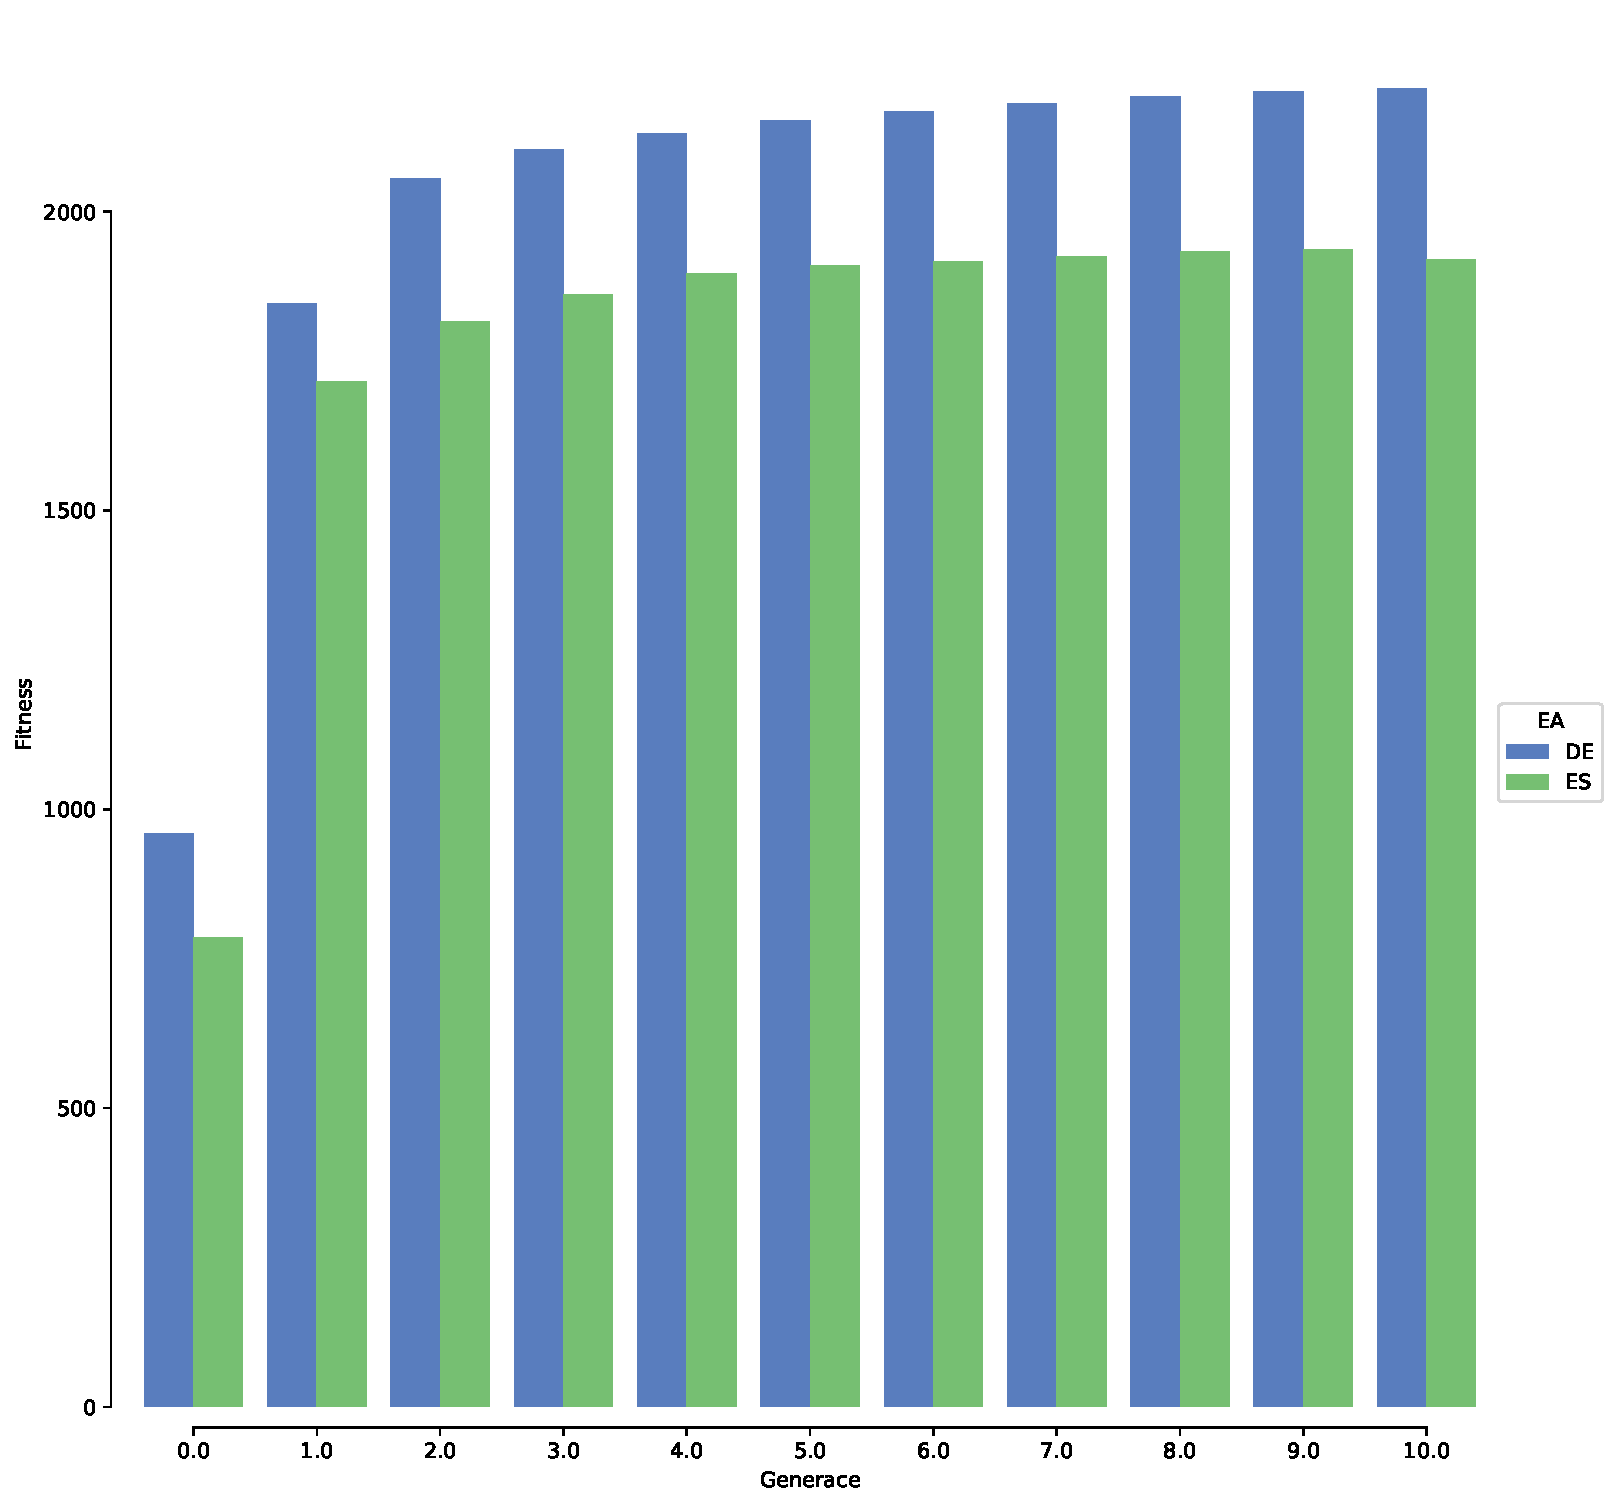
\includegraphics[width=\columnwidth]{../img/WoodMap/DEvsES/WCuttorWalkMem}
		\caption{ Scout chůze - porovnání průměrné fitness ES a DE}
		\label{obr04:WalkESvsDE}
	\end{figure}
	\begin{figure}[p]
		\centering
		\begin{subfigure}{.5\textwidth}
			\centering
			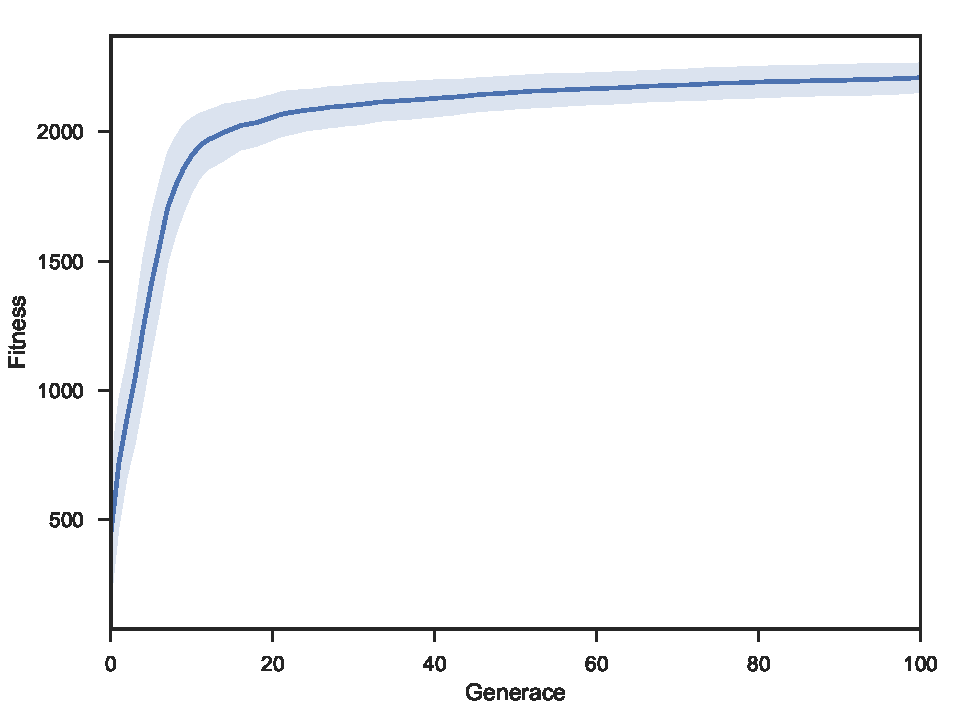
\includegraphics[width=\linewidth]{../img/WoodMap/DE/WCuttorWalkMem}
			\caption{DE}
			\label{obr04:WalkDE}
		\end{subfigure}%
		\begin{subfigure}{.5\textwidth}
			\centering
			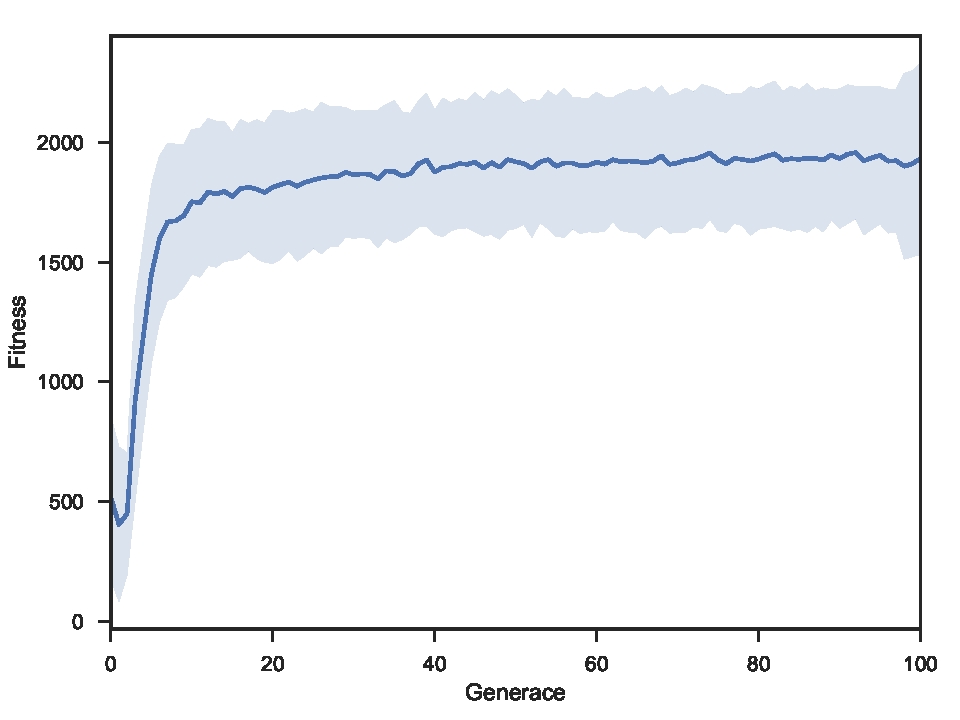
\includegraphics[width=\linewidth]{../img/WoodMap/ES/WoodWalkES}
			\caption{ES}
			\label{obr04:WalkES}
		\end{subfigure}
		\caption{Scout chůze - průběh fitness }
		\label{obr04:Walk}
	\end{figure}
	\clearpage
	
	\subsubsection{Worker chůze - nastavení experimentu}
	Worker chůze aplikuje podobný postup jako v předchozím experimentu na Worker roboty. Jen jsem nehodnotil počet nalezených stromů, ale do každé mapy jsem umístil už zpracované stromy. Roboti tedy byli oceněni za nalezení právě tohoto dřeva. Opět fitness funkce nutí roboty, co nejvíce se rozprostřít po mapě a navíc ještě vyhýbat se nepokáceným stromům.
	 	\begin{table}[h]\centering
		\begin{tabular}{l@{\hspace{1.5cm}}D{.}{,}{3.2}D{.}{,}{1.2}D{.}{,}{2.3}}
			\toprule
			& \mc{} & \mc{}\\
			\pulrad{\textbf{Vlastnost:}} & \mc{\pulrad{\textbf{Hodnota:}}}\\
			\midrule
			Roboti:     & Worker-4 \\
			Počet generací: & 1000\\
			Počet iterací map & 1000\\
			Velikost generace(DE) & 200\\
			Počet jedinců(ES) & 10\\
			Počet mutovaný potomků(ES)&20\\
			Elitismus(ES)& Ano\\
			Elitismus(DE)& Ne \\
			\bottomrule
			\multicolumn{2}{l}{}
		\end{tabular}
		\begin{tabular}{l@{\hspace{1.5cm}}D{.}{,}{3.2}D{.}{,}{1.2}D{.}{,}{2.3}}
			\toprule
			& \mc{} & \mc{}\\
			\pulrad{\textbf{Vlastnost:}} & \mc{\pulrad{\textbf{Hodnota:}}}\\
			\midrule
			Hodnota nalezeného pokáceného stromu &  100 \\
			Ostatní hodnoty: & 0\\
			Počet stromů: & 200\\
			Počet už pokácených stromů & 200\\
			\bottomrule
			\multicolumn{2}{l}{}
		\end{tabular}
		\caption{Worker chůze - nastavení experimentu}
		\label{tab04:WorkerWalk}
	\end{table}
	
	\begin{figure}[t]\centering
		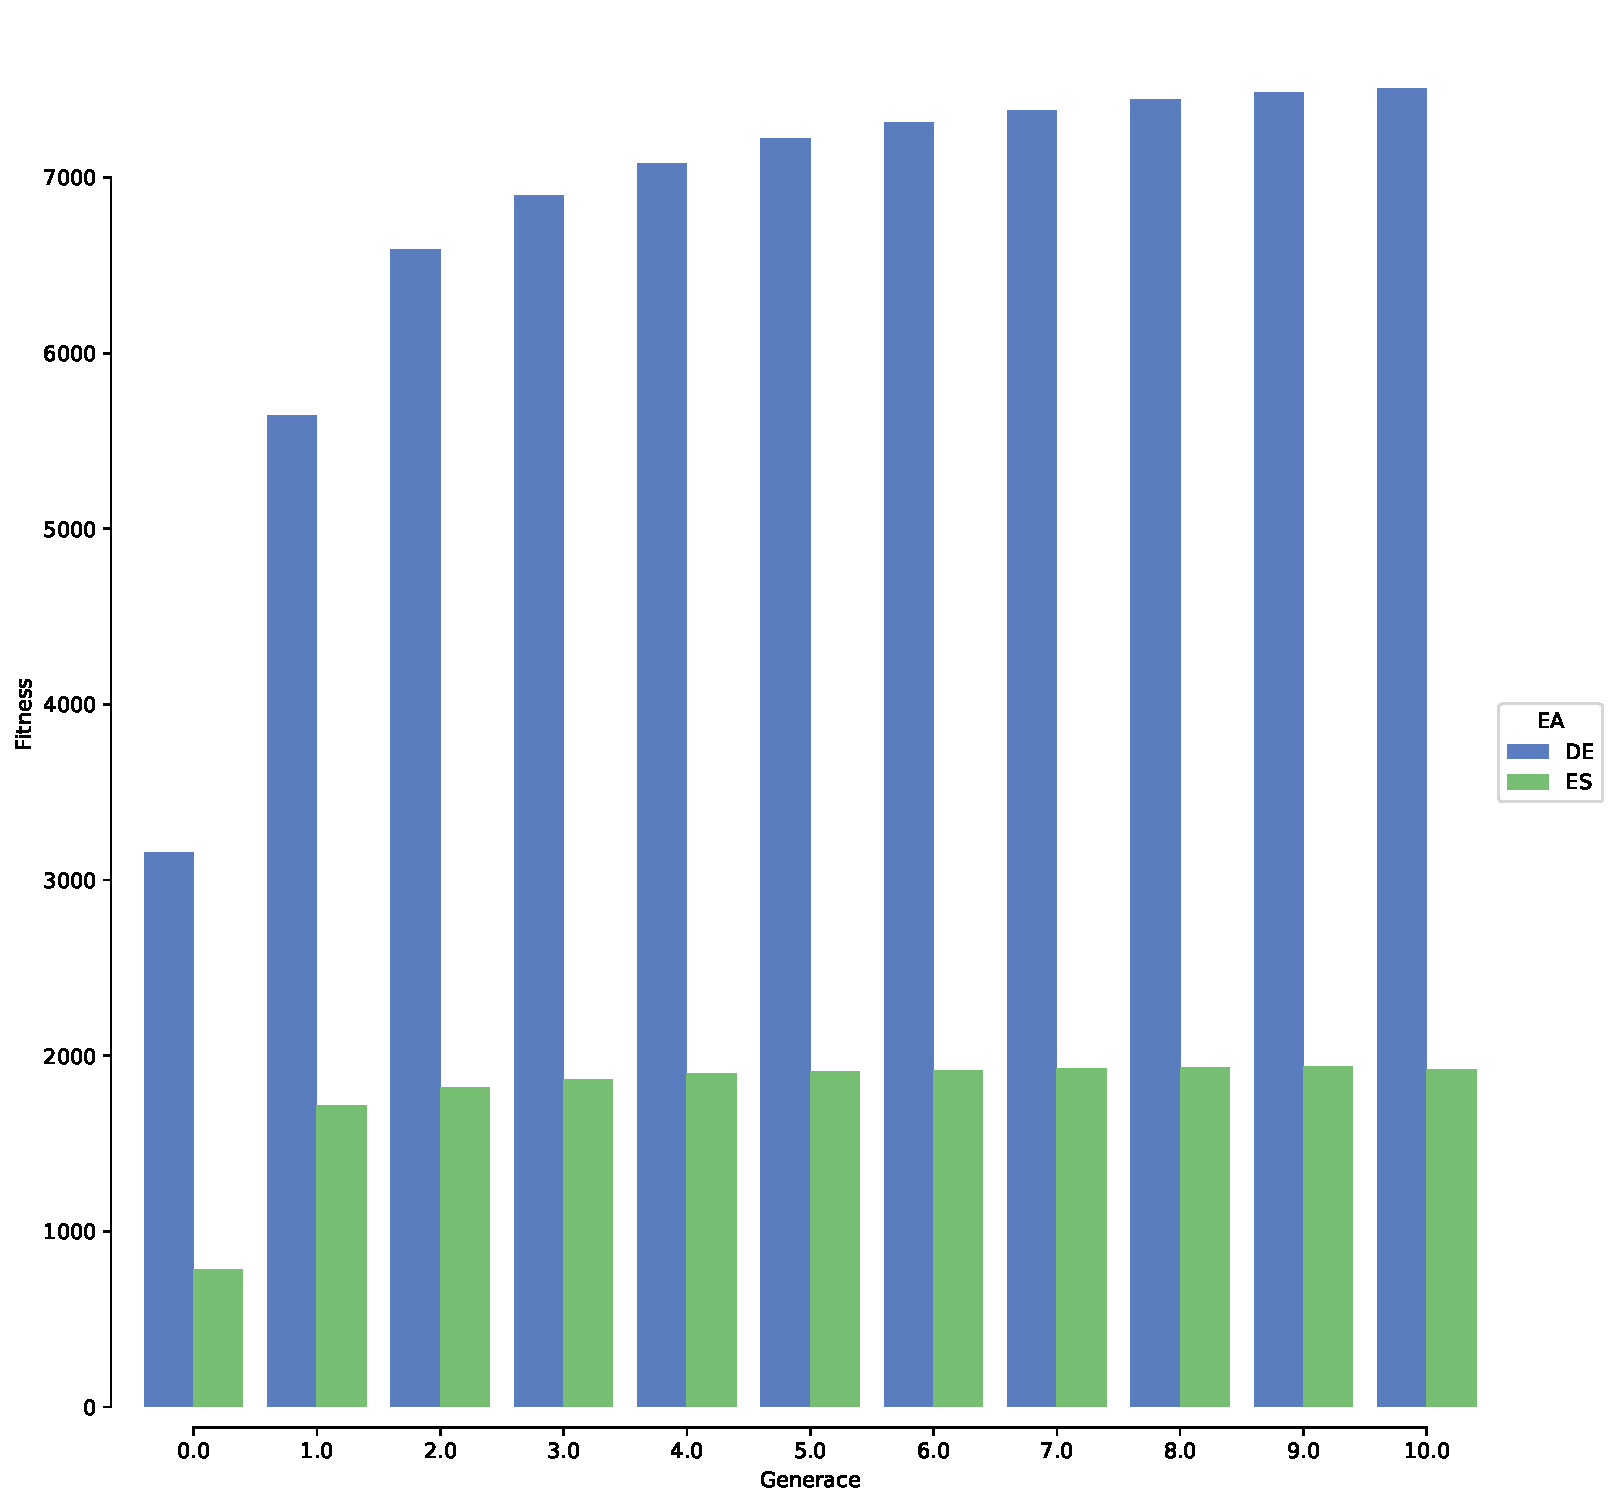
\includegraphics[width=\columnwidth]{../img/WoodMap/DEvsES/WorkerWalkMem}
		\caption{Worker chůze - porovnání průměrné fitness ES a DE}
		\label{obr04:WWalkESvsDE}
	\end{figure}
	\begin{figure}[p]
		\centering
		\begin{subfigure}{.5\textwidth}
			\centering
			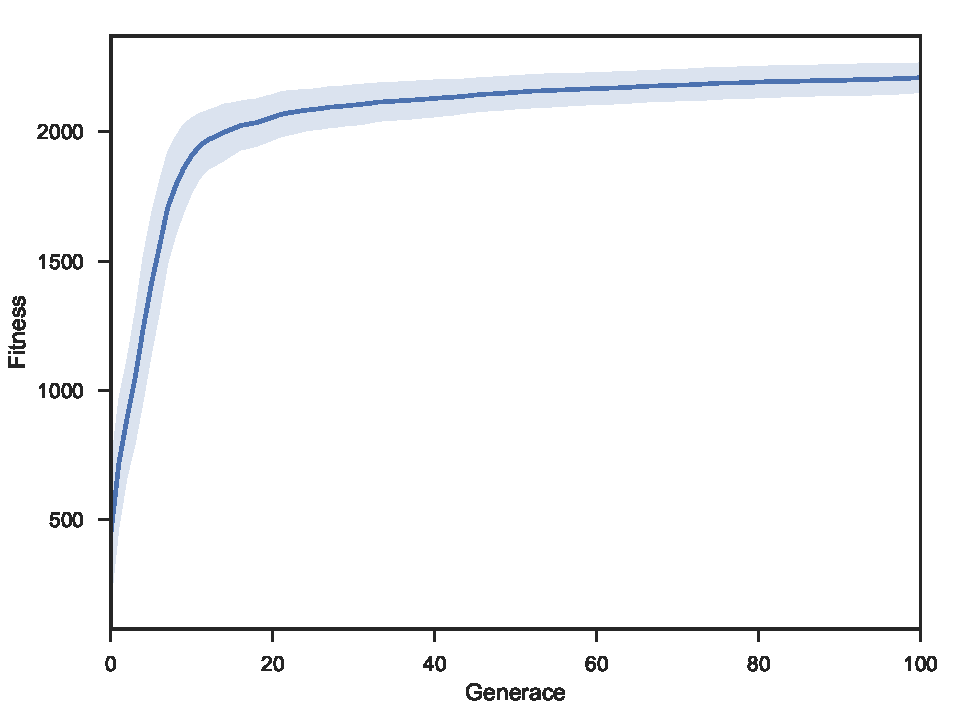
\includegraphics[width=\linewidth]{../img/WoodMap/DE/WCuttorWalkMem}
			\caption{DE}
			\label{obr04:WWalkDE}
		\end{subfigure}%
		\begin{subfigure}{.5\textwidth}
			\centering
			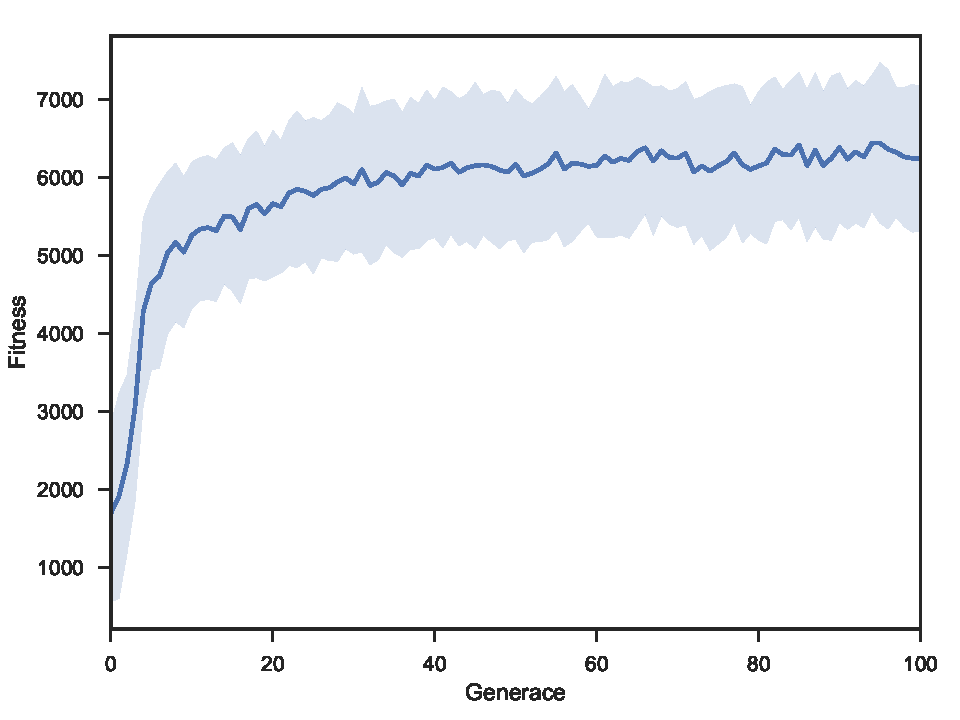
\includegraphics[width=\linewidth]{../img/WoodMap/ES/WoodWWalkES}
			\caption{ES}
			\label{obr04:WWalkES}
		\end{subfigure}
		\caption{Worker chůze - průběh fitness v rámci generací}
		\label{obr04:WWalk}
	\end{figure}

	\redo{Graf u ES je špatně,	předělat graf přepsat popisek}
	\clearpage 
	
	
	
	\subsubsection{Scout kácení - nastavení experimentu}
	Dalším úkolem pro Scout robota bylo nalezené stromy pokácet. Použil jsem tedy optimalizované neuronové sítě z experimentu Scout chůze a tentokrát přidal do fitness pozitivní body za pokácené stromy. Refaktor je o mnoho kratší než line sensory, proto pro kácení musí robot ke stromu přijet blíže. Abych ještě více vylepšil pohyb po mapě, tak každá kolize byla potrestána negativním bodem do fitness. Přesné nastavení obsahuje následující tabulka.
	\begin{table}[h]\centering
		\begin{tabular}{l@{\hspace{1.5cm}}D{.}{,}{3.2}D{.}{,}{1.2}D{.}{,}{2.3}}
			\toprule
			& \mc{} & \mc{}\\
			\pulrad{\textbf{Vlastnost:}} & \mc{\pulrad{\textbf{Hodnota:}}}\\
			\midrule
			Roboti:     & Scout-5 \\
			Počet generací: & 1500\\
			Počet iterací map & 1000\\
			Velikost generace(DE) & 200\\
			Počet jedinců(ES) & 10\\
			Počet mutovaný potomků(ES)&20\\
			Elitismus(ES)& Ano\\
			Elitismus(DE)& Ne \\
			\bottomrule
			\multicolumn{2}{l}{}
		\end{tabular}
		\begin{tabular}{l@{\hspace{1.5cm}}D{.}{,}{3.2}D{.}{,}{1.2}D{.}{,}{2.3}}
			\toprule
			& \mc{} & \mc{}\\
			\pulrad{\textbf{Vlastnost:}} & \mc{\pulrad{\textbf{Hodnota:}}}\\
			\midrule
			Hodnota nalezeného stromu &  1000\\
			Hodnota pokáceného stromu & 10000\\
			Hodnota kolize & -1\\
			Ostatní hodnoty: & 0\\
			Počet stromů: & 400\\
			Počet už pokácených stromů & 0\\
			\bottomrule
			\multicolumn{2}{l}{}
		\end{tabular}
		\caption{Scout kácení - nastavení experimentu}
	\end{table}
	
	\begin{figure}[t]\centering
		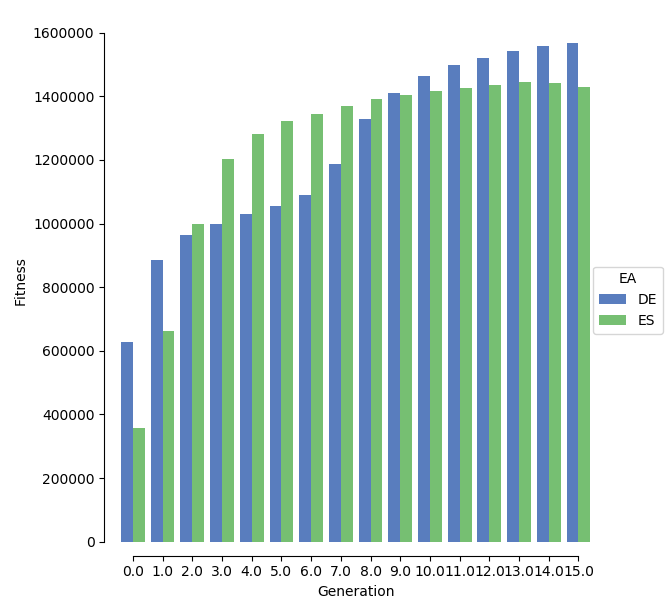
\includegraphics[width=\columnwidth]{../img/WoodMap/DEvsES/WCuttorCutMem}
		\caption{Scout kácení - porovnání průměrné fitness ES a DE}
		\label{obr04:CutESvsDE}
	\end{figure}
	Dále můžete vidět grafy popisující průběh fitness u DE, ES a porovnání jejich průměrné fitness. Z \ref{obr04:CutDE} můžeme vyčíst, že použité DE více cílí na exploataci a ES na exploraci. DE jsou díky tomu mnohem náchylnější k uvíznutí v lokálním optimu.  Fitness se v tomto případě skládá ze dvou složek, pro jedince bylo mnohem jednodušší stromy objevovat a náhodou nějaké pokácet. V prvních 650 generacích DE se tedy drží tento trend a pak se objeví jedinci, kteří cílí na kácení. Toto chování se rychle rozšířilo a fitness celé populace okolo 700. generace prudce vzrostla. Zatímco fitness v ES rostla postupně, ale nedosáhla tak vysoké úrovně jako DE. Nejlepší jedinci pokácí více než 60\% stromů. 
	\begin{figure}[p]
		\centering
		\begin{subfigure}{.5\textwidth}
			\centering
			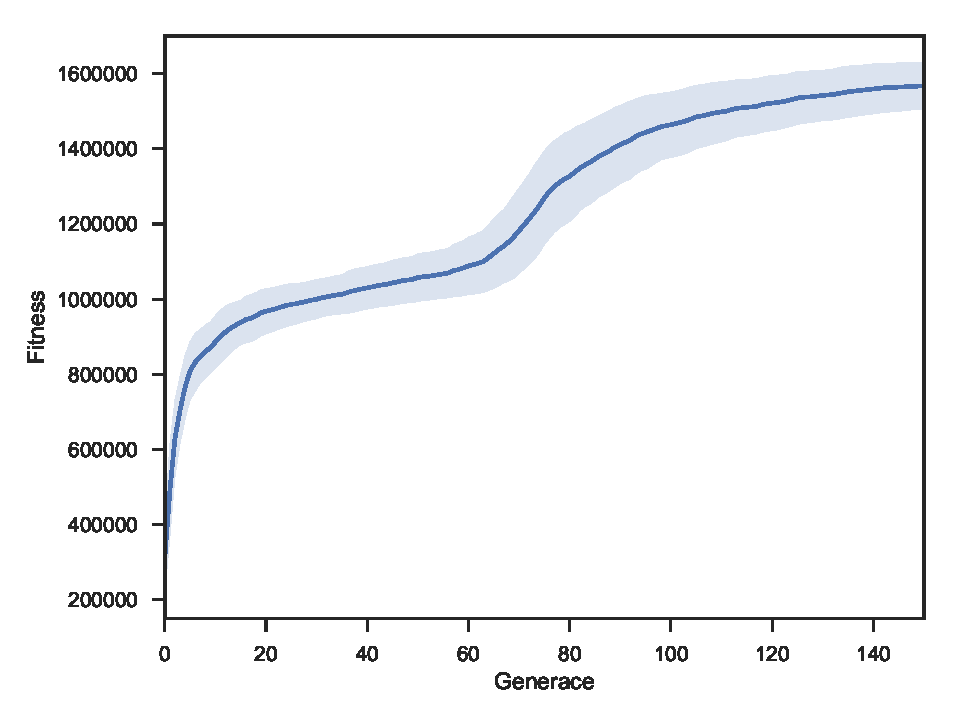
\includegraphics[width=\linewidth]{../img/WoodMap/DE/WCuttorCutMem}
			\caption{DE}
			\label{obr04:CutDE}
		\end{subfigure}%
		\begin{subfigure}{.5\textwidth}
			\centering
			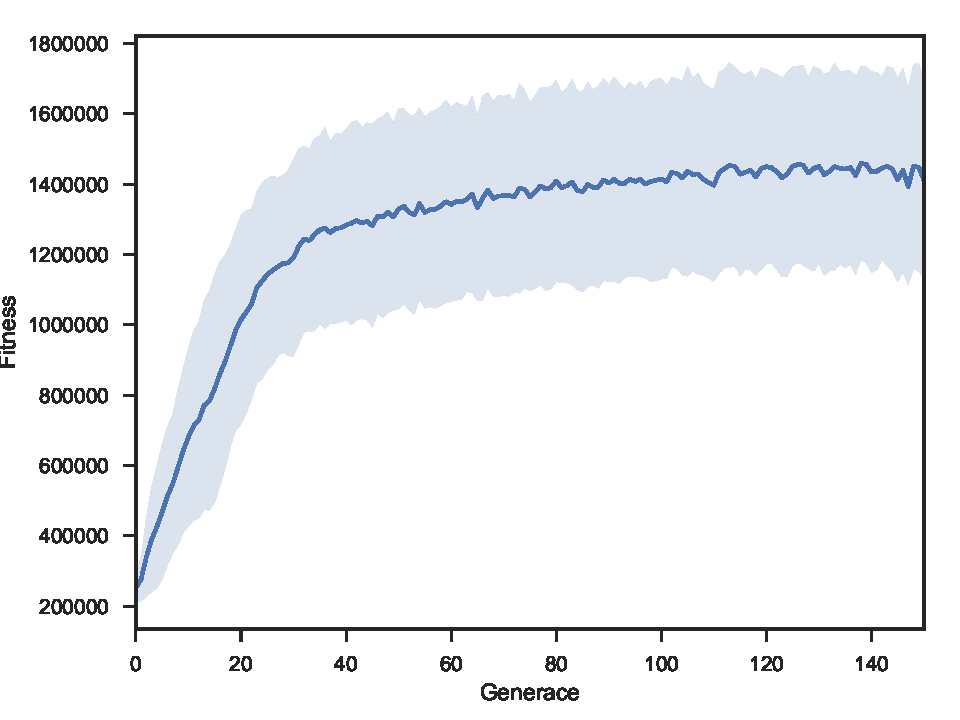
\includegraphics[width=\linewidth]{../img/WoodMap/ES/WoodCutES}
			\caption{ES}
			\label{obr04:CutES}
		\end{subfigure}
		\caption{Scout kácení - průběh fitness v rámci generací}
		\label{obr04:Cut}
	\end{figure}
	\clearpage
	
	\subsubsection{Worker sbírání - nastavení experimentu}
	\begin{table}[h]\centering
		\begin{tabular}{l@{\hspace{1.5cm}}D{.}{,}{3.2}D{.}{,}{1.2}D{.}{,}{2.3}}
			\toprule
			& \mc{} & \mc{}\\
			\pulrad{\textbf{Vlastnost:}} & \mc{\pulrad{\textbf{Hodnota:}}}\\
			\midrule
			Roboti:     & Worker-4 \\
			Počet generací: & 2000\\
			Počet iterací map & 1000\\
			Velikost generace(DE) & 200\\
			Počet jedinců(ES) & 10\\
			Počet mutovaný potomků(ES)&20\\
			Elitismus(ES)& Ano\\
			Elitismus(DE)& Ne \\
			\bottomrule
			\multicolumn{2}{l}{ }
		\end{tabular}
		\par 
		\begin{tabular}{l@{\hspace{1.5cm}}D{.}{,}{3.2}D{.}{,}{1.2}D{.}{,}{2.3}}
			\toprule
			& \mc{} & \mc{}\\
			\pulrad{\textbf{Vlastnost:}} & \mc{\pulrad{\textbf{Hodnota:}}}\\
			\midrule
			Hodnota nalezeného pokáceného stromu &  100 \\
			Hodnota uloženého dřeva & 1010\\
			Hodnota dřeva v kontejneru & 1000\\
			Hodnota jiné entity v kontejneru & -100\\
			Hodnota kolize & -1\\
			Ostatní hodnoty: & 0\\
			Počet stromů: & 200\\
			Počet už pokácených stromů & 200\\
			\bottomrule
			\multicolumn{2}{l}{}
		\end{tabular}
		\caption{Worker sbírání - nastavení experimentu}
	\end{table}
	\begin{figure}[t]\centering       
		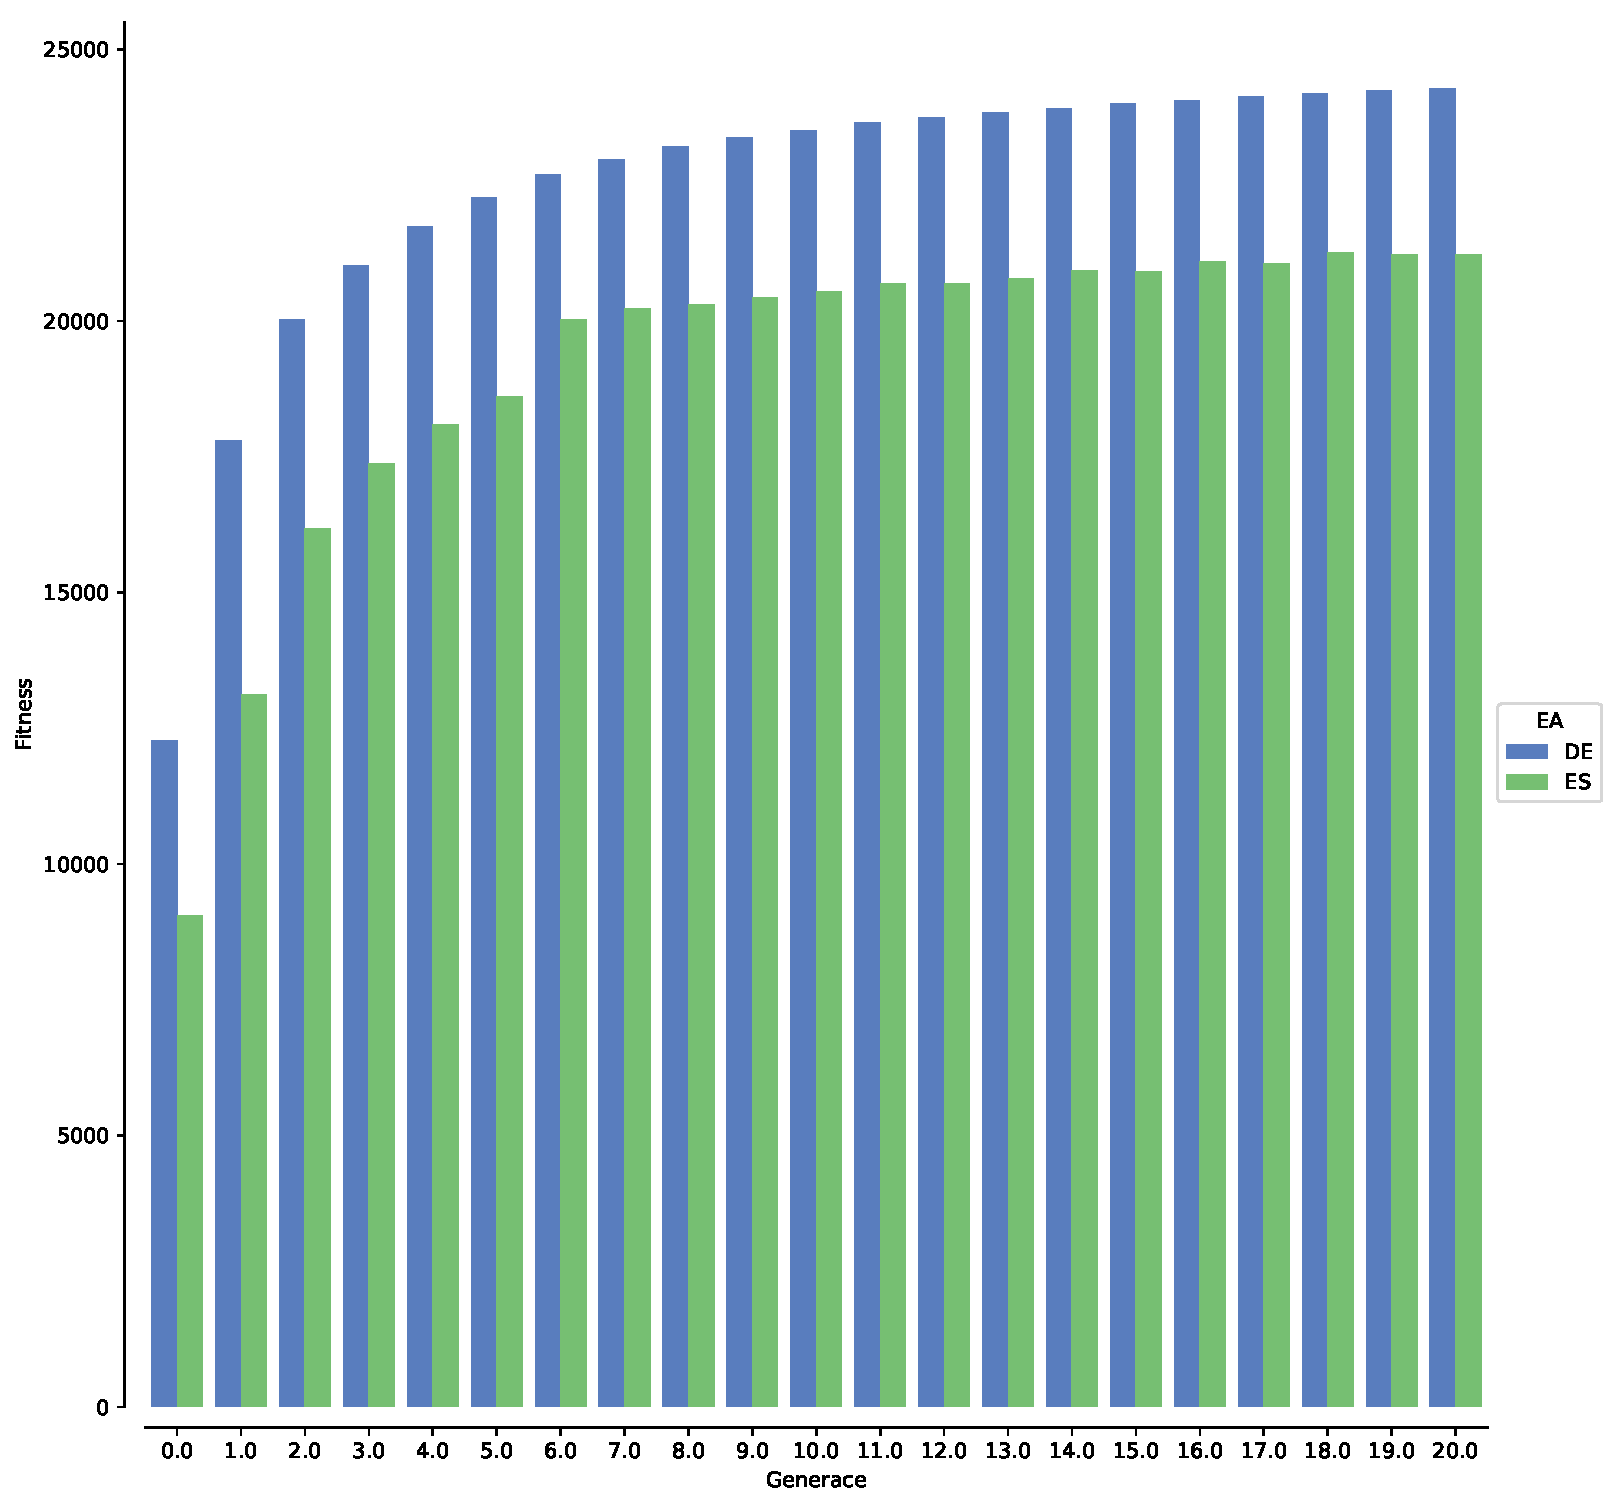
\includegraphics[width=\columnwidth]{../img/WoodMap/DEvsES/WorkerPickUpMem}
		\caption{ Worker sbírání - porovnání průměrné fitness ES a DE}
		\label{obr04:PickupESvsDE}
	\end{figure}
	\redo{Opravit obrázky
	}\begin{figure}[p]
		\centering
		\begin{subfigure}{.5\textwidth}
			\centering
			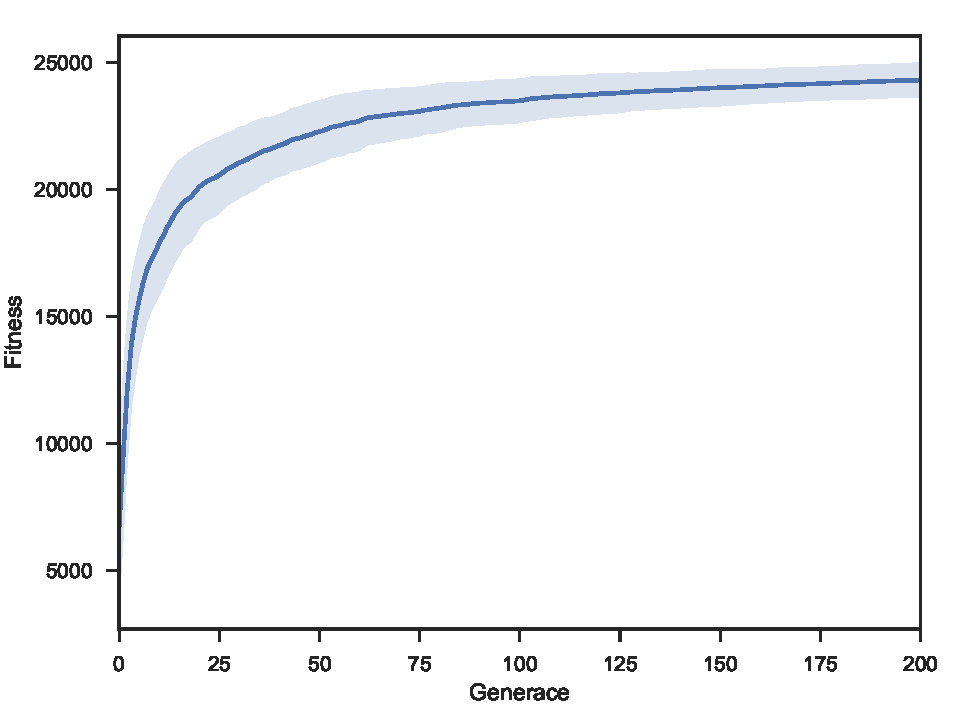
\includegraphics[width=\linewidth]{../img/WoodMap/DE/WorkerPickUpMem}
			\caption{DE}
			\label{obr04:PickupDE}
		\end{subfigure}%
		\begin{subfigure}{.5\textwidth}
			\centering
			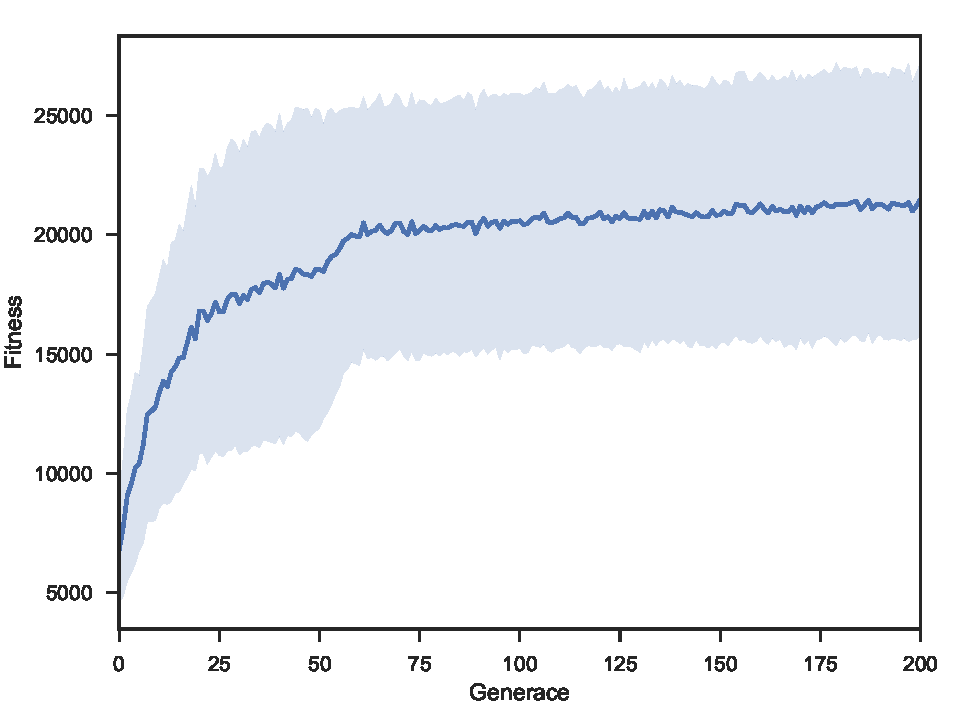
\includegraphics[width=\linewidth]{../img/WoodMap/ES/WoodPickupES}
			\caption{ES}
			\label{obr04:PickupES}
		\end{subfigure}
		\caption{Worker sbírání - průběh fitness v rámci generací}
		\label{obr04:Pickup}
	\end{figure}
	\clearpage
	\subsubsection{Worker ukládání doprostřed  - nastavení experimentu}
	\begin{table}[h]\centering   
		\begin{tabular}{l@{\hspace{1.5cm}}D{.}{,}{3.2}D{.}{,}{1.2}D{.}{,}{2.3}}
			\toprule
			& \mc{} & \mc{}\\
			\pulrad{\textbf{Vlastnost:}} & \mc{\pulrad{\textbf{Hodnota:}}}\\
			\midrule
			Roboti:     & Worker-4 \\
			Počet generací: & 2000\\
			Počet iterací map & 2000\\
			Velikost generace(DE) & 200\\
			Počet jedinců(ES) & 10\\
			Počet mutovaný potomků(ES)&20\\
			Elitismus(ES)& Ano\\
			Elitismus(DE)& Ne \\
			\bottomrule
			\multicolumn{2}{l}{ }
		\end{tabular}
		\par 
		\begin{tabular}{l@{\hspace{1.5cm}}D{.}{,}{3.2}D{.}{,}{1.2}D{.}{,}{2.3}}
			\toprule
			& \mc{} & \mc{}\\
			\pulrad{\textbf{Vlastnost:}} & \mc{\pulrad{\textbf{Hodnota:}}}\\
			\midrule
			Hodnota nalezeného pokáceného stromu &  100 \\
			Hodnota uloženého dřeva & 1000\\
			Hodnota dřeva v kontejneru & 100\\
			Hodnota jiné entity v kontejneru & -100\\
			Hodnota kolize & -1\\
			Ostatní hodnoty: & 0\\
			Počet stromů: & 200\\
			Počet už pokácených stromů & 200\\
			\bottomrule
			\multicolumn{2}{l}{}
		\end{tabular}
		\caption{Worker ukládání doprostřed  - nastavení experimentu}
	\end{table}
	\begin{figure}[t]\centering
		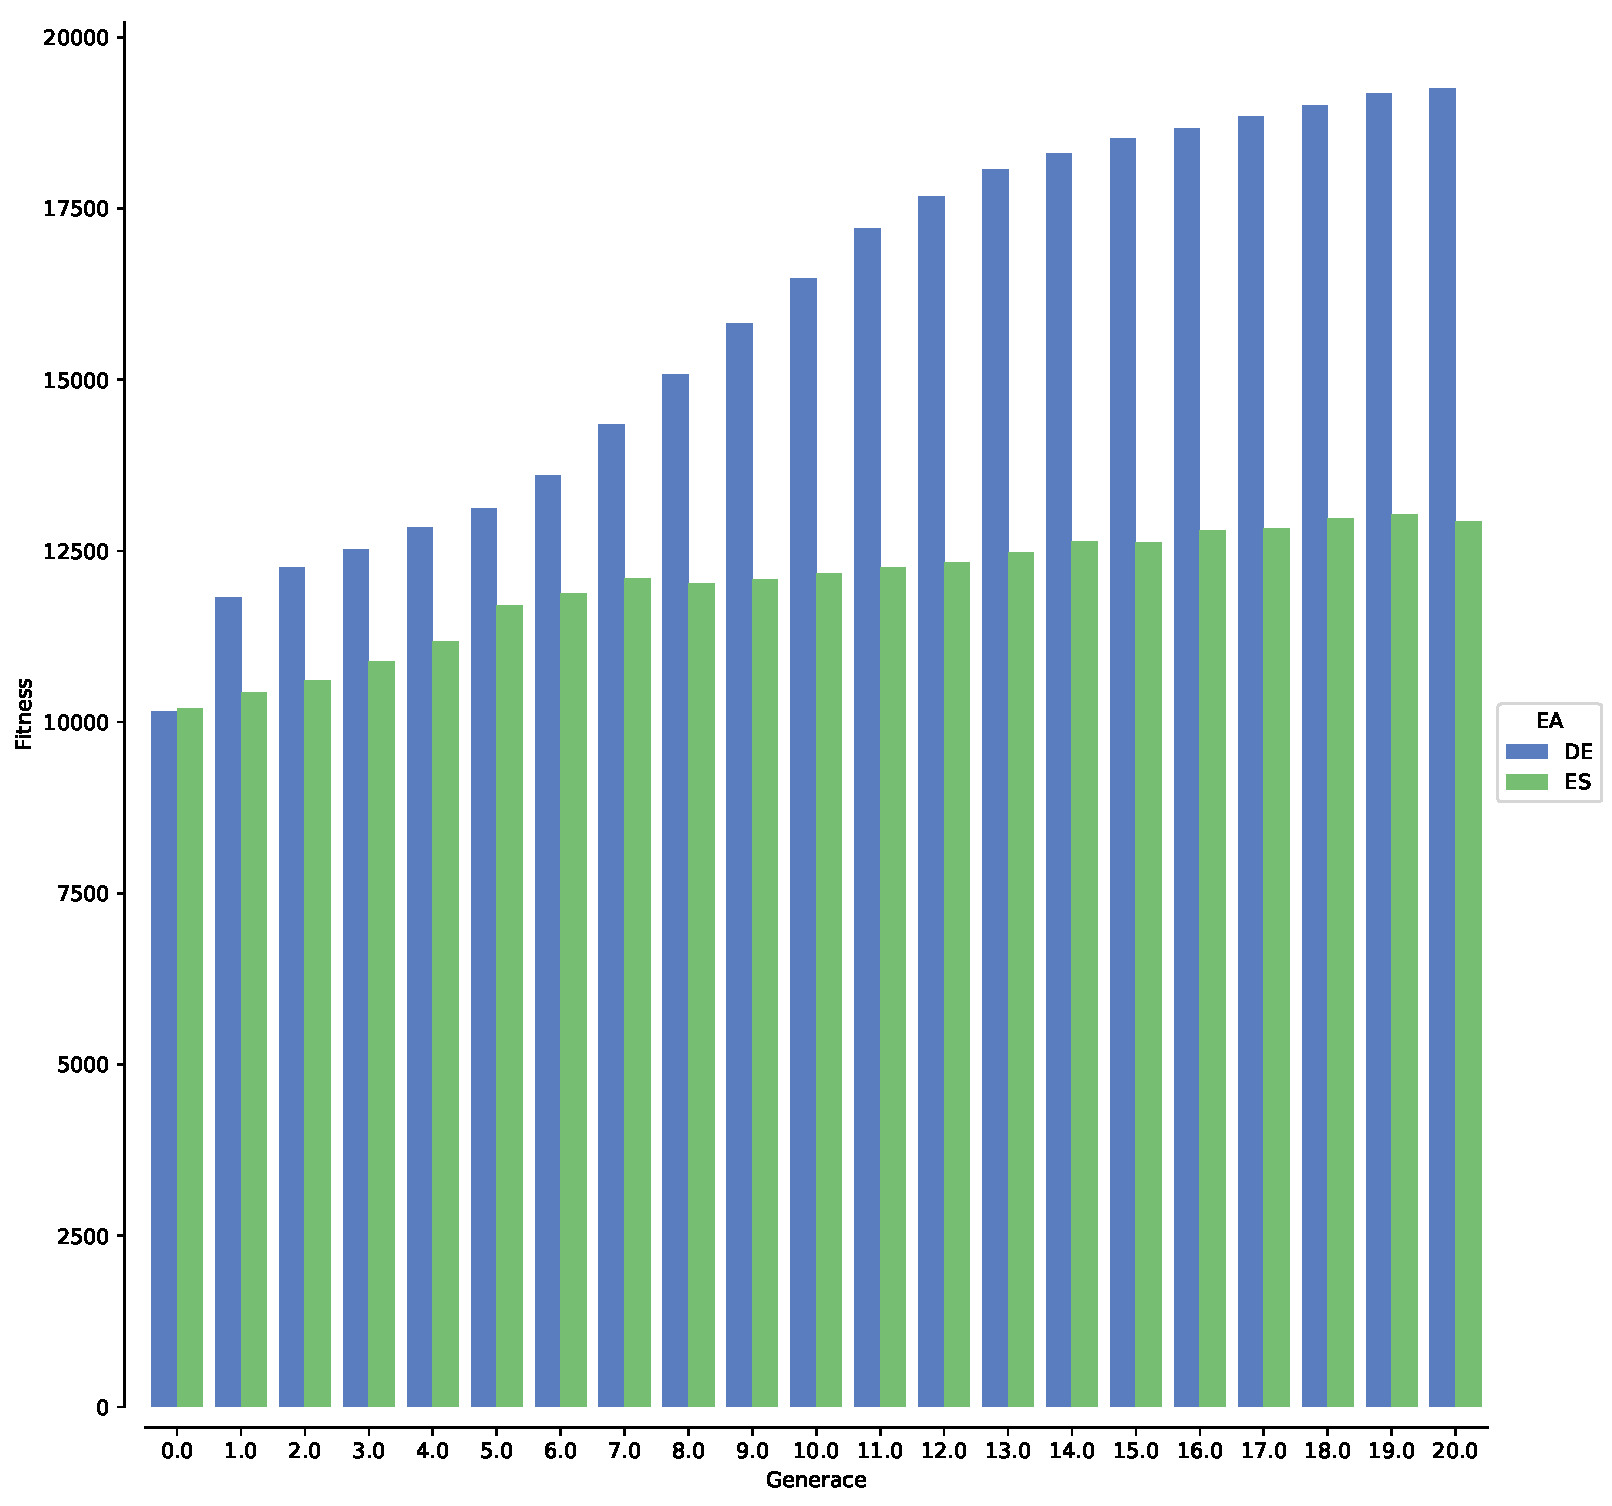
\includegraphics[width=\columnwidth]{../img/WoodMap/DEvsES/WorkerStockMem}
		\caption{Worker ukládání doprostřed  - porovnání průměrné fitness ES a DE}
		\label{obr04:StockESvsDE}
	\end{figure}
	\redo{Opravit obrázky
	}\begin{figure}[p]
		\centering
		\begin{subfigure}{.5\textwidth}
			\centering
			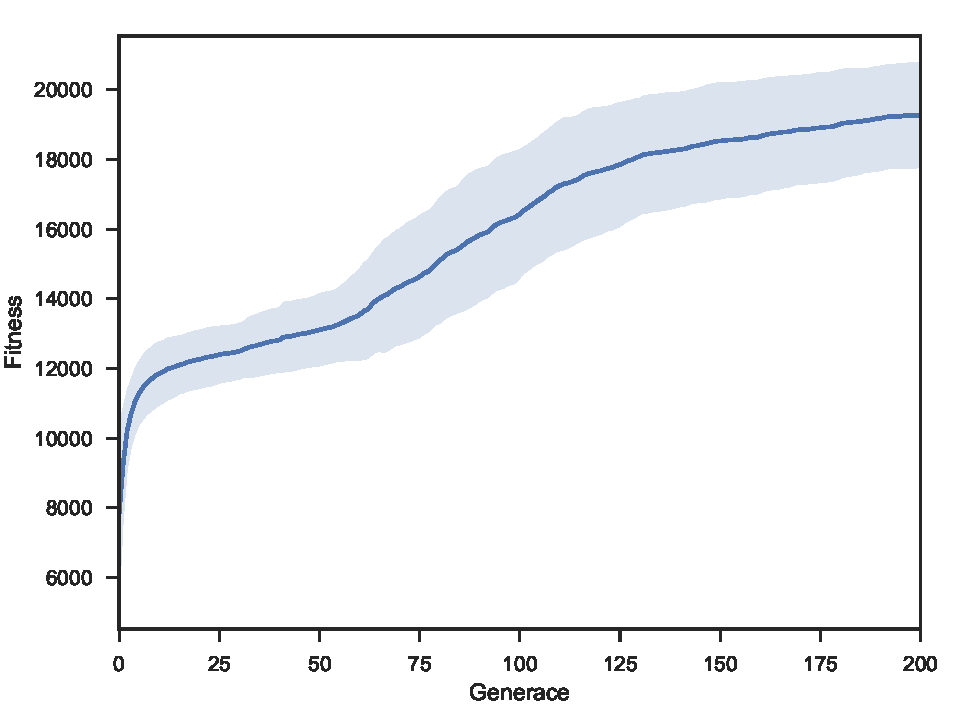
\includegraphics[width=\linewidth]{../img/WoodMap/DE/WorkerStockMem}
			\caption{DE}
			\label{obr04:StockDE}
		\end{subfigure}%
		\begin{subfigure}{.5\textwidth}
			\centering
			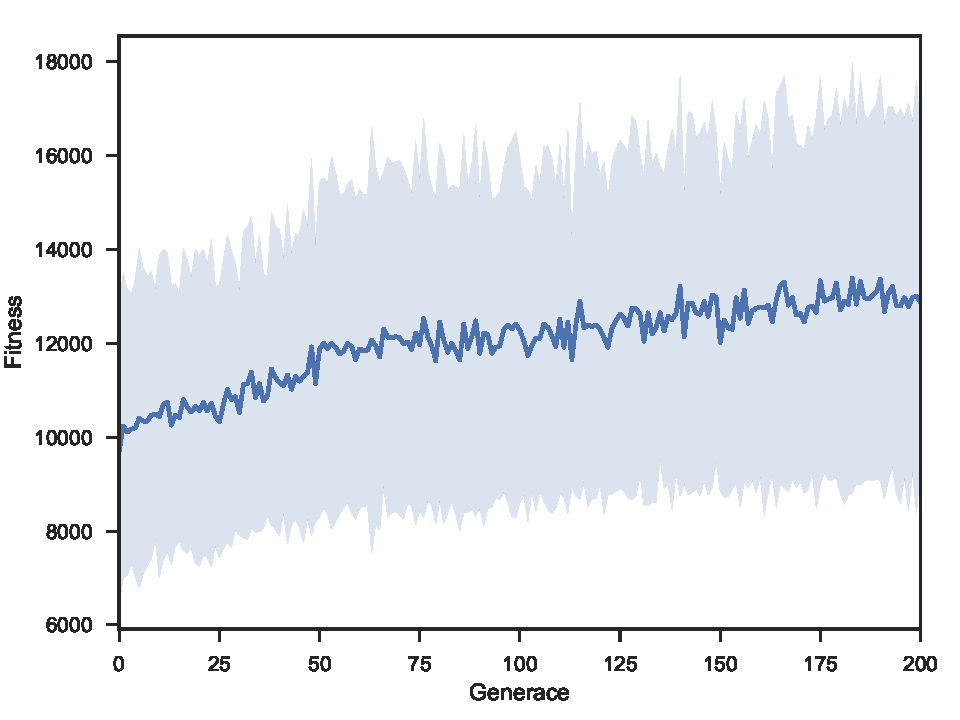
\includegraphics[width=\linewidth]{../img/WoodMap/ES/WoodStockES}
			\caption{ES}
			\label{obr04:StockES}
		\end{subfigure}
		\caption{Worker ukládání doprostřed  - Průběh fitness v rámci generací}
		\label{obr04:Stock}
	\end{figure}
	\clearpage
	\subsubsection{Kooperace  hlavní úkol  - nastavení experimentu}
	\begin{table}[h]\centering   
		\begin{tabular}{l@{\hspace{1.5cm}}D{.}{,}{3.2}D{.}{,}{1.2}D{.}{,}{2.3}}
			\toprule
			& \mc{} & \mc{}\\
			\pulrad{\textbf{Vlastnost:}} & \mc{\pulrad{\textbf{Hodnota:}}}\\
			\midrule
			Roboti: & Scout-5, Worker-4 \\
			Počet generací: & 4000\\
			Počet iterací map & 2000\\
			Velikost generace(DE) & 200\\
			Počet jedinců(ES) & 10\\
			Počet mutovaný potomků(ES)&20\\
			Elitismus(ES)& Ano\\
			Elitismus(DE)& Ne \\
			\bottomrule
			\multicolumn{2}{l}{}
		\end{tabular}
		\par 
		\begin{tabular}{l@{\hspace{1.5cm}}D{.}{,}{3.2}D{.}{,}{1.2}D{.}{,}{2.3}}
			\toprule
			& \mc{} & \mc{}\\
			\pulrad{\textbf{Vlastnost:}} & \mc{\pulrad{\textbf{Hodnota:}}}\\
			\midrule
			Hodnota nalezeného pokáceného stromu &  100 \\
			Hodnota uloženého dřeva & 1000\\
			Hodnota dřeva v kontejneru & 100\\
			Hodnota jiné entity v kontejneru & -100\\
			Hodnota kolize & -1\\
			Ostatní hodnoty: & 0\\
			Počet stromů: & 400\\
			Počet už pokácených stromů & 0\\
			\bottomrule
			\multicolumn{2}{l}{}
		\end{tabular}
			\caption{Kooperace  hlavní úkol  - nastavení experimentu}
	\end{table}
	\redo{Opravit obrázky}
	\clearpage
	
		\begin{figure}[t]\centering
		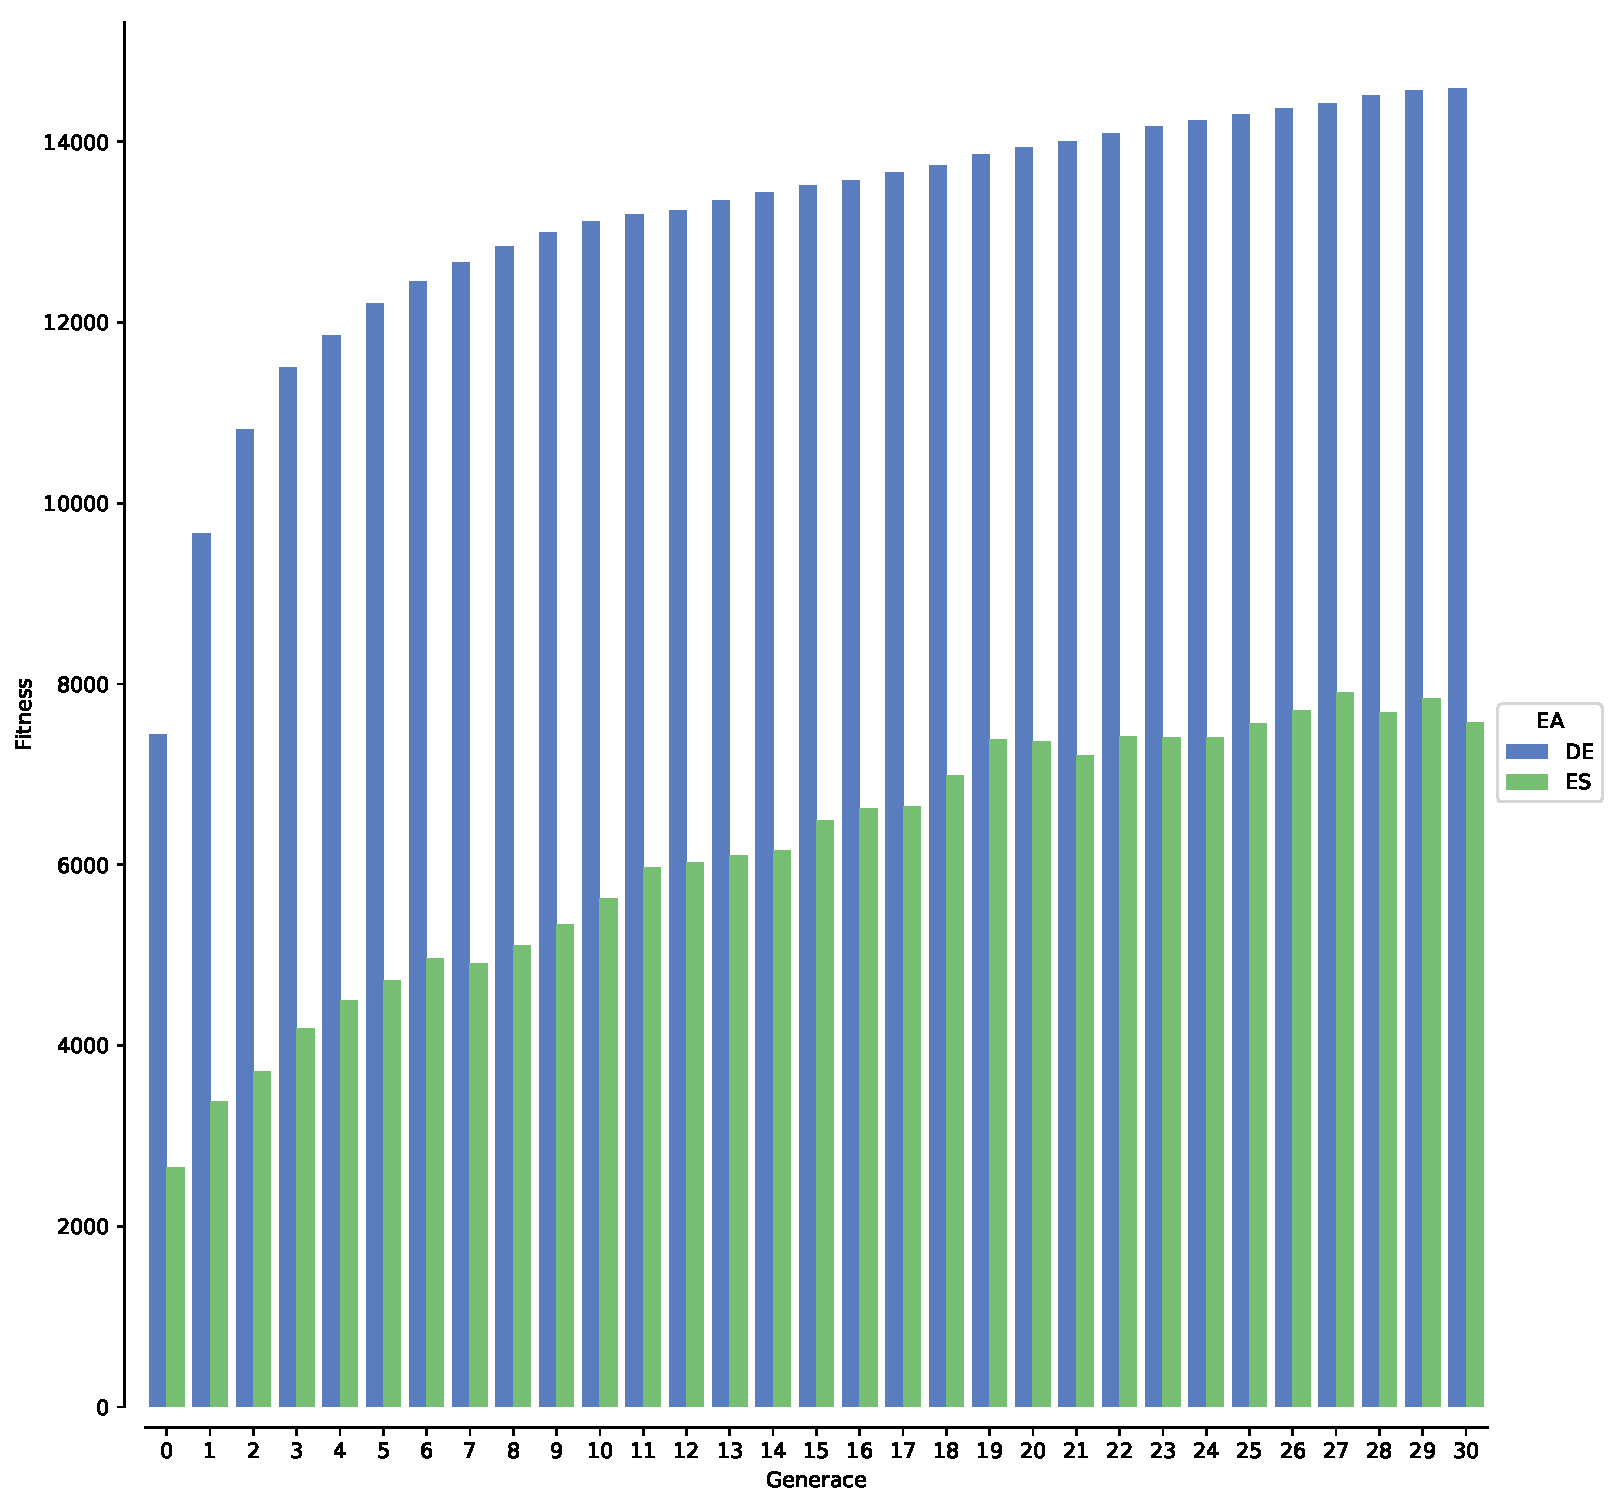
\includegraphics[width=\columnwidth]{../img/WoodMap/DEvsES/WoodCoopMem}
		\caption{Kooperace  hlavní úkol  - porovnání průměrné fitness ES a DE}
		\label{obr04:CoopESvsDE}
	\end{figure}
	\begin{figure}[p]
		\centering
		\begin{subfigure}{.5\textwidth}
			\centering
			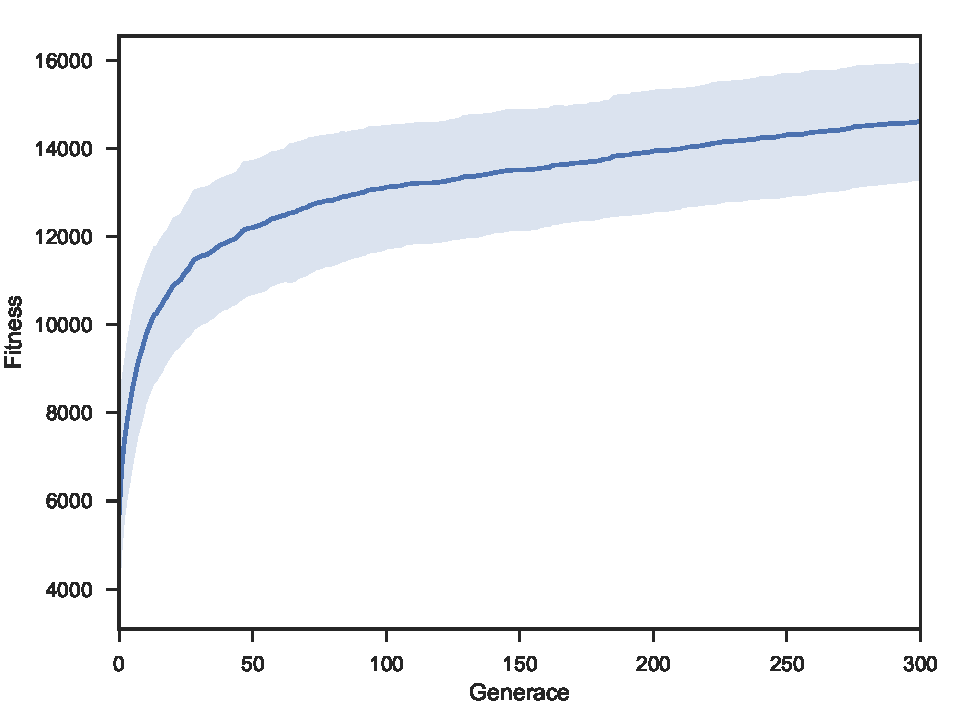
\includegraphics[width=\linewidth]{../img/WoodMap/DE/WoodCoopMem}
			\caption{DE}
			\label{obr04:CoopDE}
		\end{subfigure}%
		\begin{subfigure}{.5\textwidth}
			\centering
			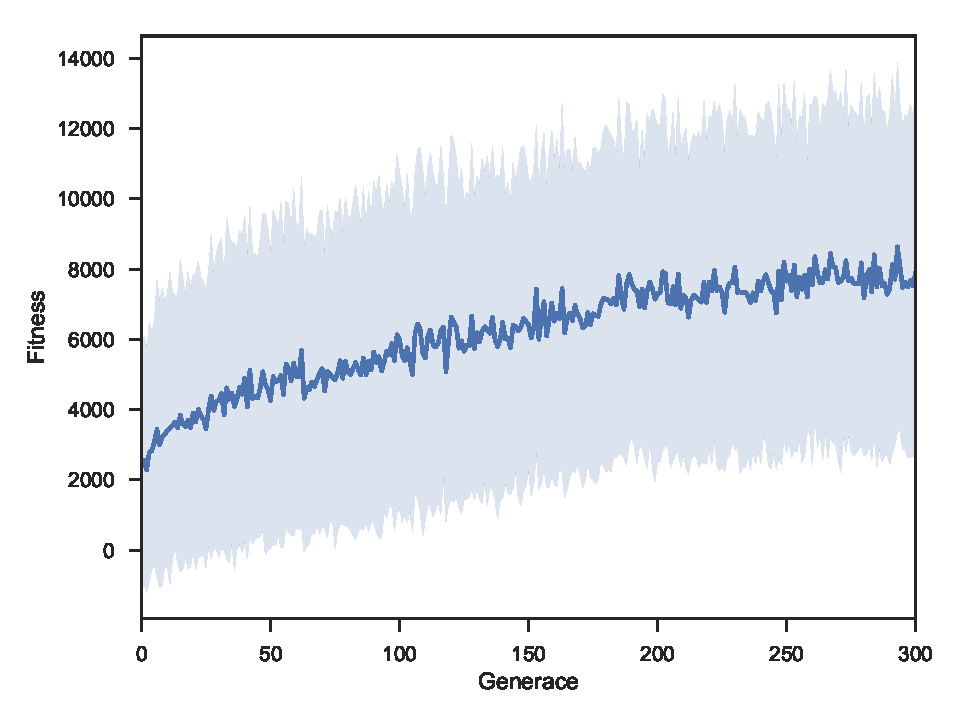
\includegraphics[width=\linewidth]{../img/WoodMap/ES/WoodCoopES}
			\caption{ES}
			\label{obr04:CoopES}
		\end{subfigure}
		\caption{Kooperace  hlavní úkol  - průběh fitness v rámci generací}
		\label{obr04:Coop}
	\end{figure}
	\clearpage
	
	\subsection{Výsledky Experimentu}
	Výsledkem posloupnosti všech podúkolů vzniklo poměrně velmi komplexní chování. Finální neuronové sítě ať u Worker robotů, či Scout robotů se zvládají vyhýbat překážkám. Scout roboti kácí stromy, které naleznou. Worker roboti nakládají zpracované dřevo, pokud na něj narazí, když zachytí signál úložiště, tak vyloží aktuální náklad. Některá chování byla také schopna předejít zaseknutí o nějaký shluk objektů, pokud byl  jejich pohyb vpřed neúspěšný, tak po několika pokusech roboti vycouvali a vydali se cestou okolo kritického místa. U většiny se také objevilo použití rádiových signálů jako prostředku pro největší možné rozptýlení po mapě, jakmile zachytí cizí signál vydají se opačným směrem. Průběh fitness jednotlivých podúkolů je zachycena na předchozích grafech \ref{obr04:Walk} až \ref{obr04:StockES}. 
	
	Ač se jedná o nejlepší dosažené chování objevují se nějaké nedostatky. Worker robot se občas dostane do pozice, ze které není schopen vyjet, jedná se především o kolize s vícero entitami. Tento problém by mohlo vyřešit použití vícevrstvých sítí či evolučního algoritmu evolvujícího i architekturu sítě. Skládání zpracovaného materiálu po obvodu skladiště není efektivní způsob, jak do něj naskládat maximální množství dřeva. V tomto případě jsem se snažil vylepšit tento nedostatek promítnutím vzdálenosti dřeva od středu skladiště do celkové fitness, ovšem bez znatelného zlepšení v chování. Nejspíše by bylo třeba použít rádiový senzor poskytující více informací o směru k zachycenému signálu. 
	\newpage 
	\begin{figure}[p]\centering
		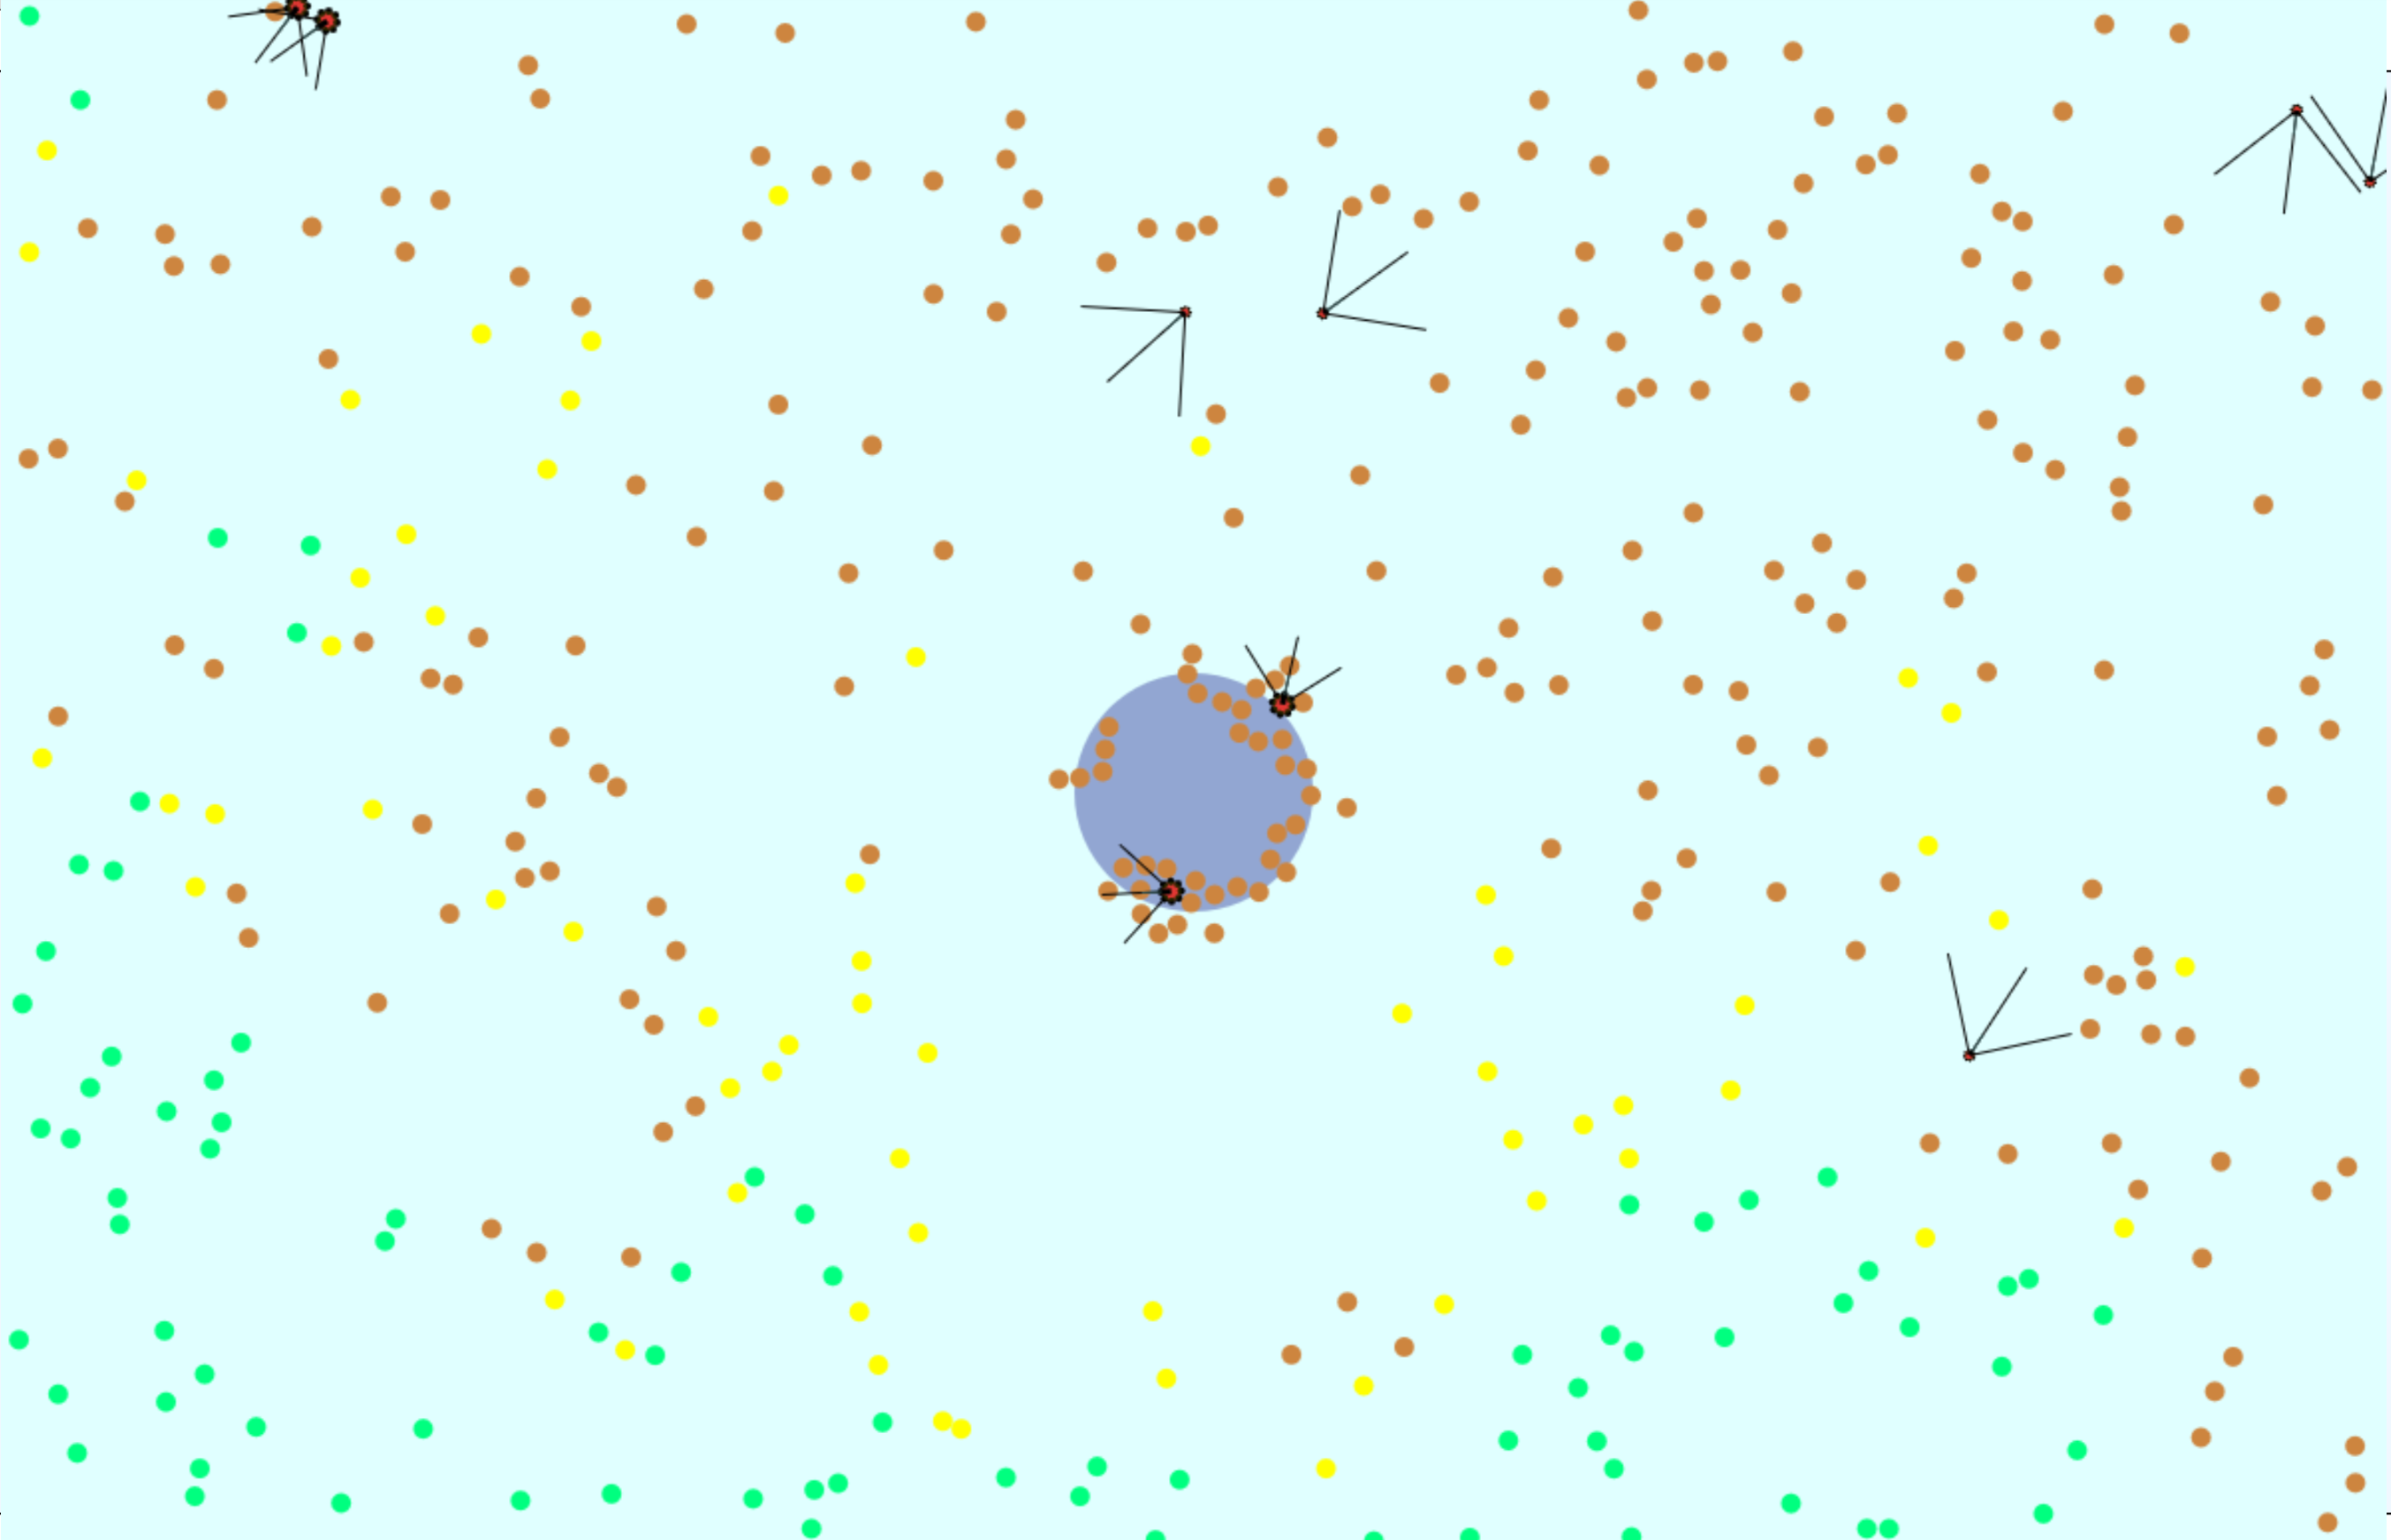
\includegraphics[width=\columnwidth]{../img/WoodMap/pictures/end.png}
		\caption{Nejlepší jedinec - 10000 iterací}
		\label{obr04:bestEnd}
	\end{figure}
	\begin{figure}[p]\centering
		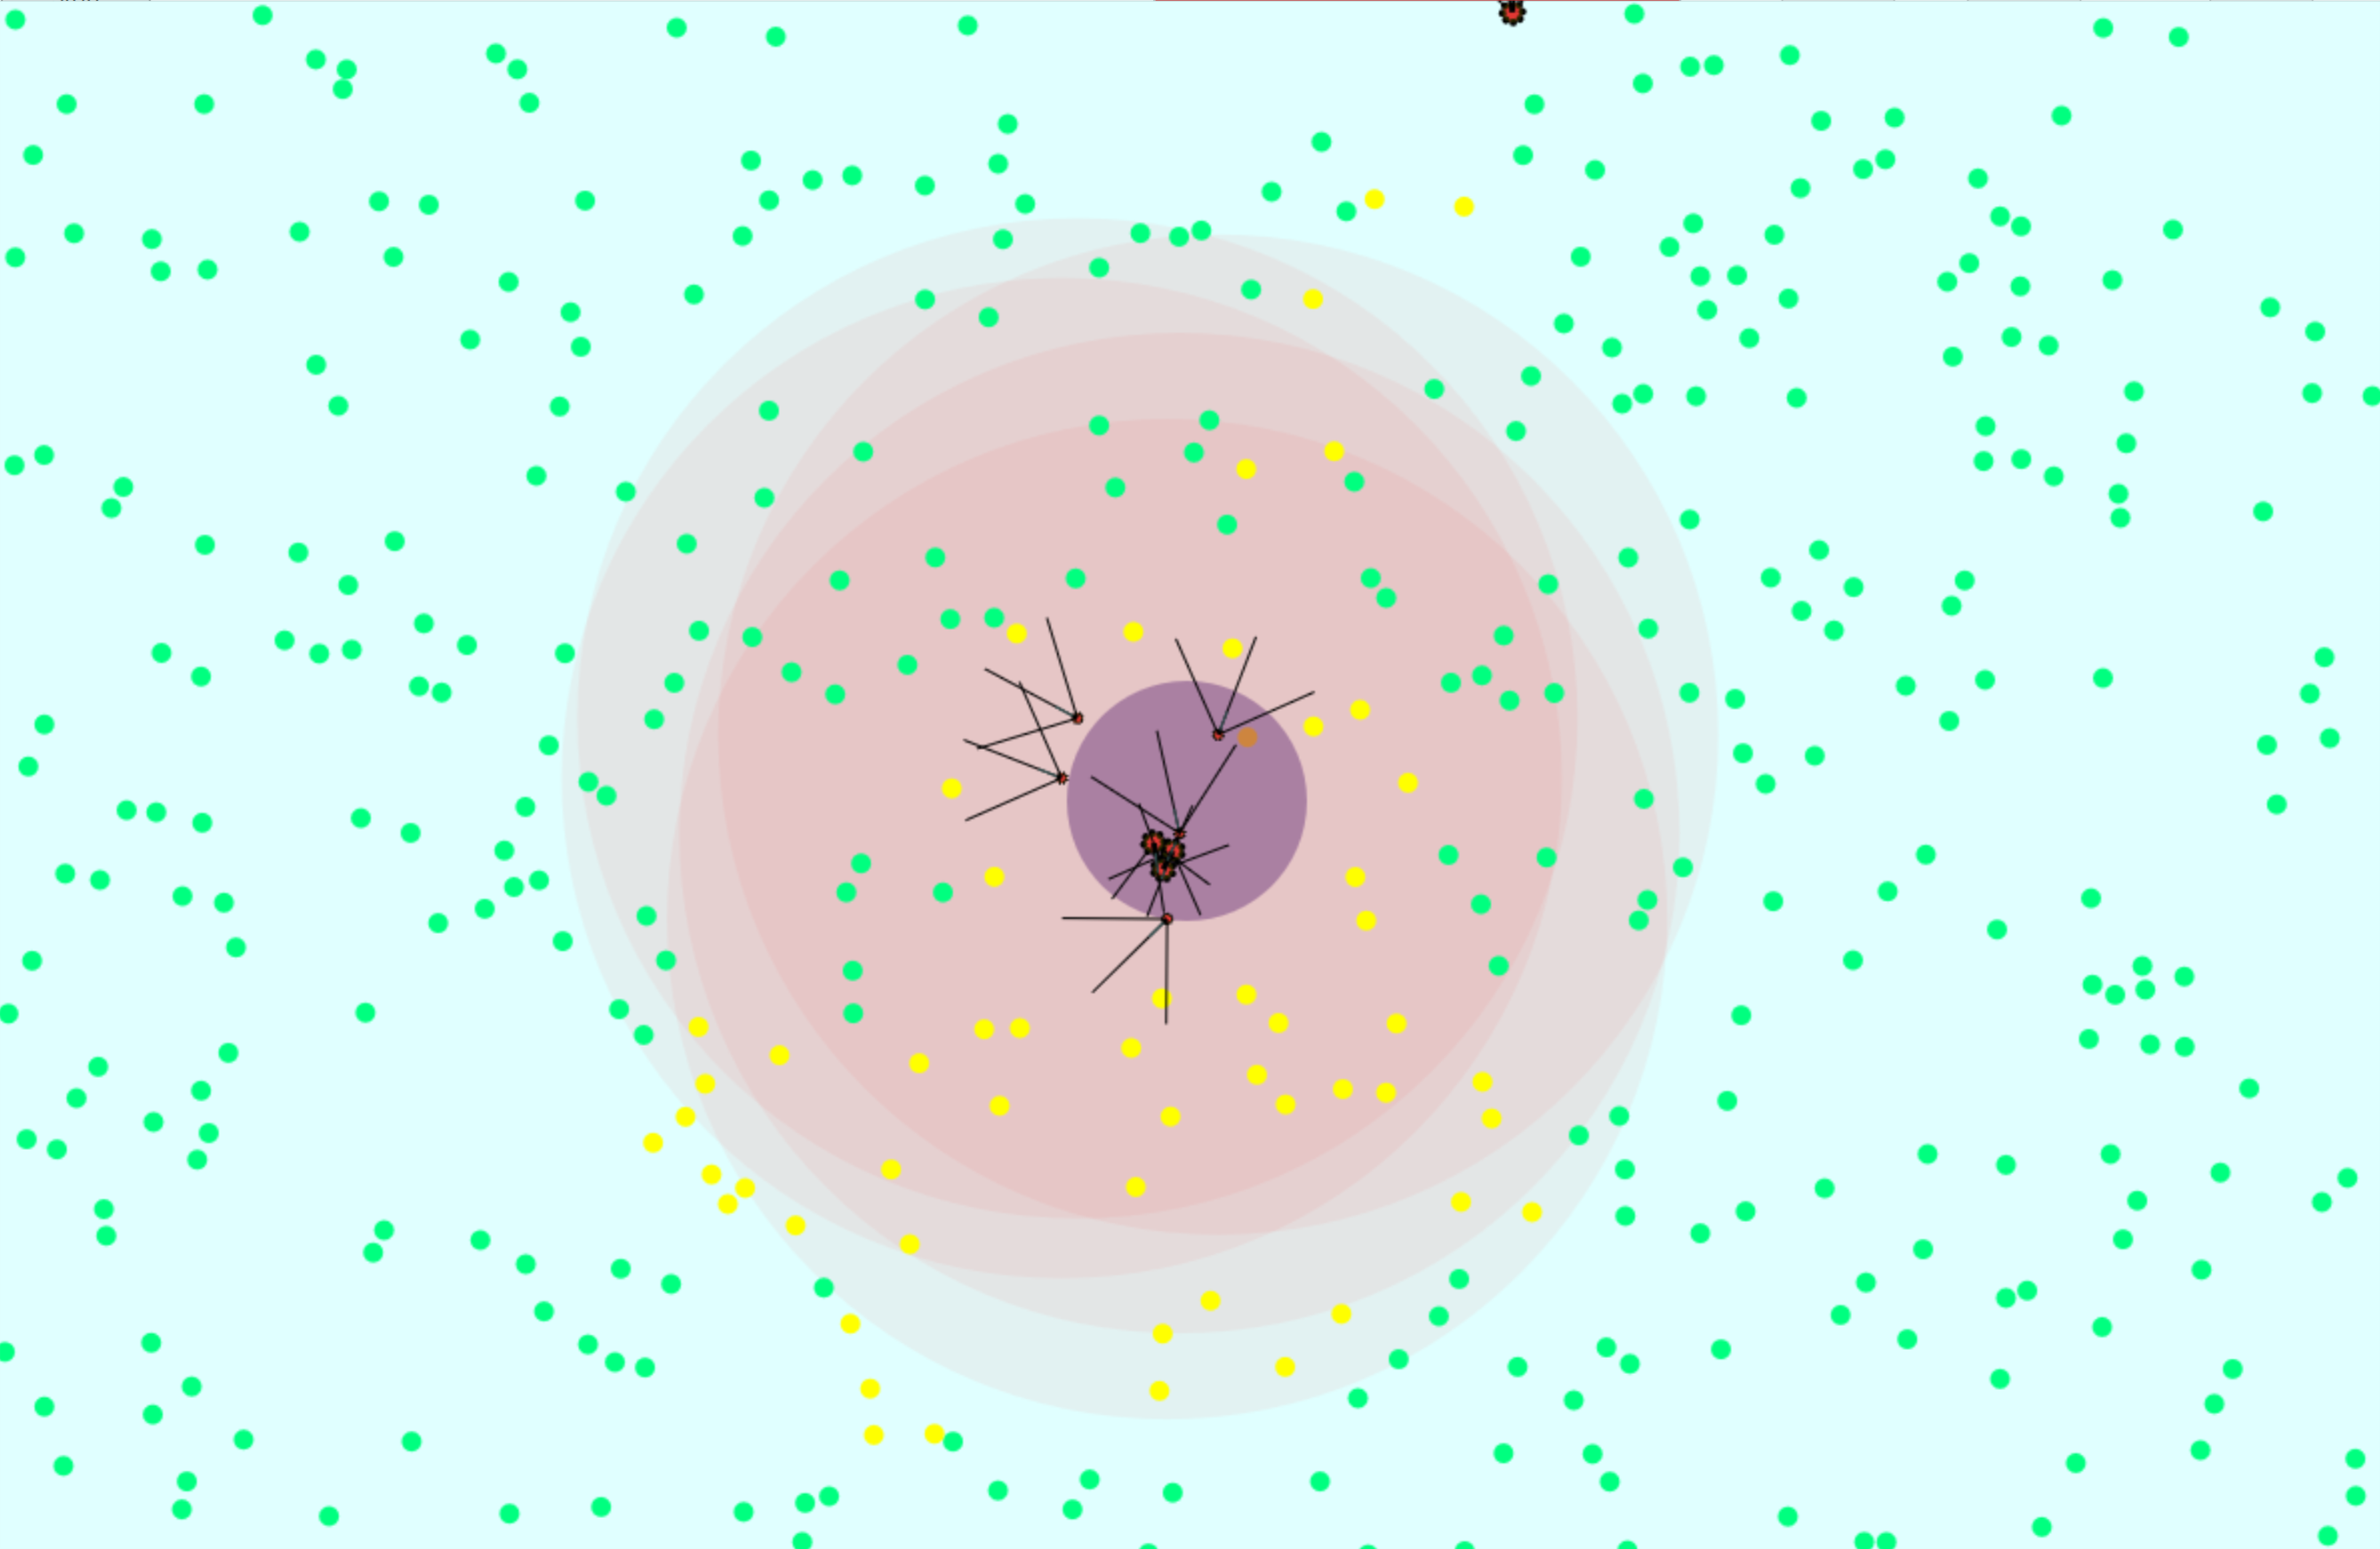
\includegraphics[width=\columnwidth]{../img/WoodMap/pictures/EndRandom.png}
		\caption{Nejlepší jedinec - 10000 iterací}
		\label{obr04:randomEnd}
	\end{figure}
	\clearpage
	\begin{table}[h]\centering   
		\begin{tabular}{l@{\hspace{1.5cm}}D{.}{,}{3.2}D{.}{,}{1.2}D{.}{,}{2.3}}
			\toprule
			& \mc{} & \mc{}\\
			Inicializační nastavení:  \\
			\midrule
			Výška & 800\\ 
			Šířka & 1200\\
			Počet iterací & 10000\\
			Počet stromů & 400\\
			Počet Scout robotů & 5\\
			Počet Worker robotů & 4\\
			\bottomrule
			\multicolumn{2}{l}{}
		\end{tabular}
		\caption{WoodScene - nastavení mapy pro statistické údaje}
	\end{table}
	\begin{table}[h]\centering   
		\begin{tabular}{l@{\hspace{1.5cm}}D{.}{,}{3.2}D{.}{,}{1.2}D{.}{,}{2.3}}
			\toprule
			& \mc{} & \mc{}\\
			Výsledky \\
			\bottomrule
			Zpracované dřevo zanechané v mapě & 225.22\\
			Stromy v mapě & 156.22\\
			Z toho nalezené & 52.84\\
			Dřevo v kontejnerech & 18.48\\
			Uskladněné dřevo & 17.56\\
			\multicolumn{2}{l}{}
		\end{tabular}
		\caption{WoodScene - průměrné výsledky nejlepšího chování pro 100 pokusů}
	\end{table}
	\paragraph{Shrnutí}
	\redo{Nějak shrnout, úplně nevím, co  by to mělo obsahovat.}
	\newpage

\redo{Předělat na stejný formát jako předchozí kapitola}
\section{Mineral Scene}
Jedná se o scénář reprezentující sběr surovin pro výrobu paliva a jeho následné využití. Figurují zde 3 rozliční roboti, všichni potřebují pro pohyb  dané množství paliva. Úspěšnost daného hejna se měří množstvím paliva. Nejmenší robot(Mineral scout) disponuje pouze senzory k exploraci prostředí a rádiovým vysílačem pro komunikaci se skupinou. Robot prostřední velikosti(Mineral Worker) se pohybuje o něco pomaleji než Mineral Scout, ale umí přesouvat objekty i více najednou. Robot pro přeměnu minerálu(,suroviny na výrobu paliva,) označen ve frameworku jako Mineral Refactor se přemisťuje nejpomaleji, má možnost přeměnit minerál na palivo. Tento scénář si bere jako inspiraci strategické hry a hypotetické přežití robotů na cizí planetě, kde si budou muset obstarat vlastní 
nerostné suroviny pro běh.

\section{Competitive Scene}
Poslední ze scénářů se týká soutěže dvou týmů(hejn) ve kterých figurují jeden malý průzkumný robot(Competitive Scout) a jeden vetší bojový robot(Competitive Fighter). Úspěšnost týmu je dána zachovanými jednotkami zdraví robotů a uděleným poškozením do nepřátelské skupiny robotů. Competitive Scout se pohybuje značně rychleji než Competitive Fighter, ale uděluje menší poškození. Což lze opět vztáhnout na chování rozdílných skupin nepřátel např. ve strategických hrách, kde se jejich chování adaptuje, co nejlépe na dané prostředí. 